\documentclass[a4paper, 12pt, openany, oneside]{book} %chose the paper size and font size. Openany ensures that all all chapters and similar may begin at any page, not only odd pages. For the introductory pages and appendices we want openany, but for chapter pages in the main content we want chapters to begin only on odd pages (right hand side). The book class ensures that the margins are automatically adjusted such that left hand pages are slightly moved to the left and vice versa at the right, which makes the thesis very readable and good looking when printed in bound book format.


% Importing document settings from our file "packages.sty"
\usepackage{packages}


\begin{document}

% Insert title page
\import{./}{title} %include the title page from the file

% % The pre-chapters
% \chapter*{Abstract} %pre-chapters should not be numbered, hence the "*"
% \pagenumbering{roman} %introductory pages should be roman
% \setcounter{page}{1}
% \addcontentsline{toc}{chapter}{Abstract} %add the chapter to the table of contents, this is not automatically added when creating unnumbered chapters (*). Add it in a chapter style, and keep all chapters on the same numberline indent regardless of number or not on the chapter
% \input{Chapters/0aAbstract} %insert the chapter text from the files

% % \chapter*{Preface}
% % \addcontentsline{toc}{chapter}{Preface} 
% % \input{Chapters/0bPreface}

% \tableofcontents
% % \addcontentsline{toc}{chapter}{\protect\numberline{}Contents}

% %add to table of contents list of figures and tables, and insert list of figures and tables
% \addcontentsline{toc}{chapter}{\protect\numberline{}\listfigurename}
% \listoffigures
% \addcontentsline{toc}{chapter}{\protect\numberline{}\listtablename}
% \listoftables


% \chapter*{Abbreviations}
% \addcontentsline{toc}{chapter}{\protect\numberline{}Abbreviations}
% \printglossary[type=\acronymtype, title={Abbreviations}]
% % \input{Chapters/02Abbreviations}
% \input{acronyms.tex}
% \newpage

% % \myemptypage
% %add an empty non-counted page by the command below in order to get the first chapter on the left hand side, if needed (check your page number so that the first chapter is on an odd page)


%%%%%%%%%%%%%%%%%%%%%%%%%%%%%%%%%%%%%%%%%%%%%%%%%%%%%%%%
% The pre-chapters
% The pre-chapters
\pagenumbering{roman}
\setcounter{page}{1}

\chapter*{AI Declaration}
\addcontentsline{toc}{chapter}{AI Declaration}
\input{Chapters/0aAIdecllaration.tex}

\chapter*{Abstract}
\addcontentsline{toc}{chapter}{Abstract}

This thesis is concerned with addressing two main questions: what is the expected lifetime of a dual spacecraft cooperative GNSS-R formation flying mission, and how accurate are its predictions adjusted for its underlying Basilisk framework prediction accuracy? To address these questions, two distinct simulators were developed, the Comparative Propagation Simulator, and the GNSS-R Formation Flight Simulator. In order to accurately estimate the formation lifetime, its operational constraints had to be modeled, including the satellite configuration, electronic power system, autonomous mode switching, attitude- and formation control. The estimated lifetime was predicted using modes derived from two simulation campaigns, studying the fuel consumption's sensitivity to the leader and follower deployment velocities, and the steady-state formation-maintenance fuel consumption, respectively. The final lifetime estimates derived from the combination of these two models were $413.6~\mathrm{days}$ and $366.5~\mathrm{days}$ for the most optimistic and pessimistic deployment cases, respectively. However, due to modelling uncertainty and observed formation drift, the estimate was evaluated to be conservative.


The Basilisk propagation configuration used in the lifetime analysis was developed as a continuation of the specialization project, where the previous exponential atmosphere model was replaced by the higher-fidelity NRLMSISE-00 atmosphere model. This thesis configuration was benchmarked against a continuously updating Skyfield-\gls{sgp4} baseline by evaluating both same-spacecraft state differences and same-formation drift differences. The same-spacecraft comparison showed that the thesis configuration diverged substantially less from the Skyfield-\gls{sgp4} reference than the specialization-project configuration. However, the same-formation comparison showed that the thesis configuration predicted larger passive leader-follower drift than the Skyfield-\gls{sgp4} baseline. Since the lifetime campaigns were therefore likely subject to higher relative drift than predicted by the comparison baseline, it supports the claim of conservative mission lifetime estimate.

\chapter*{Sammendrag}
\addcontentsline{toc}{chapter}{Sammendrag}
Denne masteroppgaven tar for seg to hovedspørsmål: hva er den forventede levetiden til et sammarbeidende GNSS-R-formasjonsflygingsoppdrag med to satellitter, og hvordan bør denne estimerte  levetiden tolkes sett i lys av prediksjonsnøyaktigheten til det underliggende Basilisk-rammeverket? For å besvare disse spørsmålene ble det utviklet to separate simulatorer: en simulator for å sammenlikne propagasjonssimuleringer, og en GNSS-R-formasjonsflygingssimulator. For å estimere levetiden til formasjonsoppdraget måtte begrensningene tilknyttet GNSS-R oppdraget modelleres, inkludert satellittkonfigurasjon, det elektriske systemet, autonom modusbytting, attityde- og formasjonskontroll. Den estimerte levetiden ble predikert ved hjelp av modeller utledet fra to simuleringsrunder, som henholdsvis undersøkte drivstofforbrukets sensitivitet for leder- og følgersatellittenes utskytningshastighet fra et delt romfartøy, og drivstofforbruket knyttet til formasjonsvedlikehold i stasjonær tilstand. De endelige levetidsestimatene, utledet ved bruk av disse modellene, var $413.6~\mathrm{dager}$ og $366.5~\mathrm{dager}$ for henholdsvis det mest optimistiske og det mest pessimistiske utskytningsscenarioet. På grunn av modelleringsusikkerhet og observert formasjonsdrift ble estimatet vurdert som konservativt.
 
Basilisk-propagasjonskonfigurasjonen som ble brukt i levetidsanalysen, ble utviklet som en videreføring av spesialiseringsprosjektet, hvor den tidligere eksponentielle atmosfæremodellen ble erstattet av NRLMSISE-00  atmosfæremodellen. Denne konfigurasjonen ble sammenlignet med en kontinuerlig oppdatert Skyfield-\gls{sgp4}-referanse ved å evaluere både tilstandsforskjeller for samme satellitt og formasjonsdriftsforskjeller. Sammenligningen av samme satellitt viste at konfigurasjonen brukt i denne masteroppgaven divergerte betydelig mindre fra Skyfield-\gls{sgp4}-referansen enn konfigurasjonen fra spesialiseringsprosjektet. Sammenligningen av formasjonsdrift viste imidlertid at konfigurasjonen i denne masteroppgaven predikerte større passiv leder-følger-drift enn Skyfield-\gls{sgp4}-referansen. Siden levetidskampanjene dermed sannsynligvis var utsatt for større relativ drift enn det som ble predikert av sammenligningsreferansen, støtter dette vurderingen av levetidsestimatet som konservativt.


\chapter*{Preface}
\addcontentsline{toc}{chapter}{Preface}
This master's thesis marks the completion of my studies in the two-year Master's Degree Program in Cybernetics and Robotics at the Norwegian University of Science and Technology (NTNU), Department of Engineering Cybernetics.

The work has been both challenging and rewarding, and has given me the opportunity to apply theory from cybernetics, orbital mechanics, simulation, and control to a complex space mission analysis problem. Developing and analyzing the Basilisk-based simulation framework has provided valuable insight into both the technical modelling process and the practical limitations that arise when building long-horizon spacecraft simulations.

I would like to express my sincere gratitude to my supervisor, Jan Tommy Gravdahl, for his guidance, feedback, and support throughout the thesis work. I would also like to thank my co-supervisor, Corrado Chiatante, for valuable discussions and academic input during the project.

A special thanks goes to Oliver Keving Hasler for valuable input related to the implementation of the simulations in Basilisk. His insights were helpful in addressing several practical modelling and implementation challenges.

Finally, I would like to thank my family, friends, and fellow students for their support, encouragement, and discussions throughout the semester.

\clearpage
% \chapter*{Contents}
\tableofcontents

\clearpage
% \chapter*{List of Figures}
\listoffigures

\clearpage
% \chapter*{List of Tables}
\listoftables

\clearpage
\chapter*{Abbreviations}
\printglossary[
    type=\acronymtype,
    title={},
    toctitle={Abbreviations}
]

\clearpage


%%%%%%%%%%%%%%%%%%%%%%%%%%%%%%%%%%%%%%%%%%%%%%%%%%%%%%%%
%Customize the layout of the main content of your thesis

\pagestyle{fancy} %set customized page style for header
\fancyhf{} %clear header and footer fields
\renewcommand{\headrulewidth}{0pt} %set to no rule
\fancyhead[LE, RO]{\thepage} %set the page number at left for even, right for odd pages
\fancyhead[RE, LO]{\leftmark} %set the chapter name at right for even, left for odd pages
%is is possible to design the header with the chapter as you wish, e.q. only the chapter or only the name, all lowercase instead etc.
%you could also design the footer if you wish, for example:
%\fancyfoot[LE, RO]{\thepage}
\setlength{\headheight}{14.49998pt} %set the header height


%%%%%%%%%%%%%%%%%%%%%%%%%%%%%%%%%%%%%%%%%%%%%%%%%%%%%%%%
%main content 
\pagenumbering{arabic}
\chapter{NOTES}
\input{Chapters/99NOTES}
\cleardoublepage

% \pagenumbering{arabic}
\chapter{Introduction}
\label{chap:introduction}
% https://www.itk.ntnu.no/emner/masteroppgave


% \section{Motivation}
% % This source "Recent Advances on Jamming and Spoofing Detection in GNSS" (saved pdf) by Rados et al. explains the what jamming/spoofing is in detail


% This has to be included in the report to make it clear to the sensors what has been done:
% \begin{itemize}
%     \item Information, software and equipment available/used
%     \item What help has been received during the work
%     \item The use of AI. The AI-declaration schema MUST be inserted on the first page after the title page
% \end{itemize}

% \subsection{FNs sustainability goals}

% \subsection{Background and motivation}

% \section{Take-aways from the specialization project}

% \subsection{Research problem}

% \subsection{Research objectives}

% \subsection{Research questions}



\section{Background \& Motivation}  

% gnss as a signal of oppertunity due to the global GNSS coverage
\gls{gnss} have become deeply embedded into our modern infrastructure with multiple constellations, such as GPS, GLONASS, Galileo and BeiDou, ensuring that four satellites are observable from the surface at any given time, thus providing worldwide coverage \cite{nasa_earthdata_gnss}. The sheer number of operational satellites that broadcast \gls{gnss} signals makes it one of the most powerful signals of opportunity for remote sensing, enabling monitoring without the need for onboard transmitters.
% Provide source for the final claim

% Launches has become cheaper, making it possible for smaller research gropus to implement space-based systems
At the same time, the space sector has recently undergone rapid changes. Launch costs have fallen significantly due to government outsourcing of launch providers to private companies, and the competitive environment it produced. This is clearly shown in figure \ref{fig:launch_cost}, where the per-kilogram launch cost has hit an all-time low with the deployment of SpaceX rockets \textit{Falcon9} and \textit{Falcon Heavy} \cite{jones2018launch_cost}. As a result, it has become increasingly feasible for universities, research groups and smaller nations to deploy space-based systems dedicated to leveraging \gls{gnss} signals for remote sensing applications. 

% Jamming and spoofing has increased recently, making it more valuable to locate the sources
In parallel with this growth, there has also been an increase in the frequency of reported intentional \gls{gnss} interference to disrupt aviation operations. The interference can be divided into separate categories characterized by their difference in method and effect: \textit{Jamming} refers to the relative high-power emission of \gls{rf} noise to block \gls{gnss} signals, while \textit{spoofing} is the transmission of signals that resemble those from real satellites, misleading the \gls{gnss} receiver to think it has a different position \cite{ffi_factsheet_2024}. The \gls{ffi} states that: "In Norway's northernmost county of Finnmark, close to the Russian border, loss of \gls{gnss} signals due to jamming occurs nearly daily. [\dots] The number of disruptions has increased significantly since Russia's invasion of Ukraine in 2022." \cite{ffi_jamming_2024}. Data from \textit{gpsjam.org} suggest that similar disruptions have been reported across Eastern Europe, the Middle East, and the Arctic \cite{gpsjam_2025}. These events highlight a broader geopolitical trend: \gls{gnss} interference is becoming more common. This places increased strategic value on systems that can detect and localize jamming and spoofing events.

% gnss-r as a promising technique for jamming/spoofing detection, and connection to SmallSat Lab
\gls{gnssr} offers a promising technique for addressing these challenges. According to Jin and Komjathy \cite{jin2010gnss-R}, Hall and Cordey \cite{hall_cordey_1988} were the first to propose that GNSS L-band reflections could be exploited in a bistatic radar configuration to retrieve ocean surface properties, laying the foundation for modern \gls{gnssr} techniques. Recent theory suggest that the same bistatic configuration can be used for surveillance of the \gls{gnss} spectrum, where multiple \gls{gnssr} satellites in formation can detect and localize sources of jamming and spoofing. This emerging use-case is one of the central research goals of NTNU SmallSat Lab's \gls{gnssr} project, which aim to develop methods for this process \cite{ntnu_smallsat_gnssr_2025}. The project currently investigates this concept through its \gls{gnssr} satellite mission study, exploring formations geometries, orbit configurations and system designs that would enable robust detection of \gls{gnss} interference sources and ships. 
% Might move the mentioning of SmallSat Lab to after the motication

% why gnss-r is dependent on accurate orbital propagation
Accurate knowledge of spacecraft position and velocity is essential for the performance of any \gls{gnssr} system. In such systems, regardless of application, the reflected \gls{gnss} signal is interpreted by comparing its time delay and Doppler shift relative to the direct signal. This process is highly sensitive to the specular reflection point's geolocation, which is given by the geometric relationship between the \gls{gnss} transmitter, the reflecting surface and the receiver. Even small errors in the satellite's propagated state shifts the estimated specular point by kilometers. Such errors can lead to misinterpretations of the delay-Doppler maps, for instance if the predicted specular point is over ocean when the true specular point occurs over land \cite{gleason2020cygnss}. 

In real missions, the satellite orbit and relative geometry within satellite formations will naturally drift over time due to orbital perturbations. During mission design, simulation tools are used to predict the satellites motion. If the simulation does not accurately model the relevant perturbations, its predicted state evolution will diverge from physically realistic behavior, eventually yielding incorrect specular point locations and misleading conclusions about the performance of the GNSS-R system. Furthermore, inaccuracies in position and velocity directly translates to uncertainty in later analyses, like coverage analysis, or formation-keeping delta-V estimation. For these reasons, a high-fidelity propagator is necessary to ensure realistic and reliable evaluations of the \gls{gnssr} system performance.

\begin{comment}
    * The wider context of why GNSS-R has become an attractive technology
        - The increasing use of satellite constellations in earth observation and RF sensing
        - Trends in small satellites and CubeSats
        - (Consider expanding on why high-fidelity simulations are important for these missions)
        - Why GNSS-R is emerging as a technique with significant potential
    
    * Narrow down to NTNU SmallSatLab's GNSS-R project. The specialization project's relation to it

    * Why formation geometry is important for GNSS-R performance
        - Especially important for expected ISL bitrate and the GNSS-R measurement resolution 

    * An explanation of why simulation accuracy matters:
        - More accurate estimations of energy required to maintain formations
        - Higher accuracy GNSS-R coverage, pointing and constellation estimations

    * Describe the currently used GNSS-R orbital simulation framework, and state explicitly that its accuracy is unverified for satellite formation-drift studies
        - Specify propagation method, what it models, what it lacks and why that is problematic for GNSS-R mission planning

    * Tie to the need for a more in-depth comparison
        - Expand on the potential consequences of unverified accuracy. 

[Note to self]
- Make sure the formation geometry importance leads into the simulation accuracy importance. The flow should be:
    1. GNSS-R performance depends on specific formation geometry
    2. Formation geometry evolves due to orbital perturbations
    3. Therefore, high-fidelity simulation is required to estimate drift and formation control needs. 

- Don't slam the current implementation too hard. Use claims from Skyfield to back up its SGP4 accuracy
\end{comment}


\section{Problem Definition}

% Insert Github Cite instead of '???', maybe
A system simulator has already been developed to support the development of SmallSat Lab's \gls{gnssr} project (cite???). The tool currently allows area coverage estimation and a detection probability analysis of a stationary maritime target, and is intended to be extended for ocean surveillance and \gls{gnss} \gls{rfi} detection in the future. As explored in the previous section, these analyses rely on accurately propagating both \gls{gnss} and \gls{gnssr} satellites to minimize their uncertainties. Currently, the simulator uses the \gls{sgp4} propagator through the Skyfield Python library for this purpose.  

The \gls{sgp4} propagator has long been the industry standard for orbit prediction, and has subsequently been the subject of thorough evaluation. Several studies document that the propagator can exhibit decreasing accuracy over longer time-horizons, particularly for formation-flight or precision geometry applications \cite{aida2013sgp4_accuracy}. This raises concerns about whether the current SGP4-based implementation is sufficiently accurate for GNSS-R studies, which are highly sensitive to orbital state errors.

\subsection{Research Questions}

This motivates a systematic verification of the Skyfield-\gls{sgp4} implementation by comparing its long-term predictions against a propagator with higher modeling fidelity. Therefore, this specialization project will support the SmallSat Lab \gls{gnssr} mission by developing such a propagator within the Basilisk simulation framework, which natively supports detailed perturbation models and allows for controlled comparisons with Skyfield-\gls{sgp4}. The study uses this capability to evaluate the differences between the propagators and evaluate their implications for \gls{gnssr} mission analysis. As a result, the project is guided by three research questions:
\begin{itemize}
    \item a
 \end{itemize}
 % Alternatively: How do differences in simulated translational states affect downstream orbital and formation analyses
 % Alternatively: 1. How accurate are Skyfield SGP4 orbital predictions over longer time horizons?
 Answering these questions will support the project's goal of guaranteeing the reliability and accuracy of orbital propagation tools used for \gls{gnssr} small-satellite formation studies in future mission design.

\begin{comment}
    * Describe the already implemented propagator for gnss-r analyses

    * Define the core problem: How do different orbital propagation methods and perturbation effects influence satellite formations over time? 

    * Problem statement
    
    * Research question
        - Numerical precision of same-configuration simulations:   
            What is the numerical difference between the two simulation frameworks with the exact same simulation configuration? (same disturbances modelled, same integration time, same everything.)
        - Extended perturbation effects:   
            How does including additional orbital perturbations effect the numerical difference between the two simulation frameworks over time?
        - Computational performance:   
            How does the computational time differ between the simulation frameworks?

    * Sub-tasks (I don't feel like this section is really necessary)
        - Model orbital disturbance effects

        - Implement the two simulation frameworks 
\end{comment}


\section{Overall Method}
\begin{comment}
    * This needs to be filled out when I have more information, but from chat:

        * Introduce methodological approach: deterministic numerical simulation, model-by-model isolation, etc. Examples that COULD fit:
            - "comparative simulation study"
            - "Controlled scenario with fixed ICs"
            - "Pairwise comparison under identical perturbation models"

        * State clearly that both simulators will be initialized identically

        * Describe the experiment design

    * Describe the tools used for simulator design, and result verification
\end{comment}


\section{Scope \& Limitations}
This specialization project focuses on evaluating the long-term orbital propagation accuracy of two distinct simulation frameworks, Skyfield-\gls{sgp4} and a high-fidelity Basilisk propagator, in the context of \gls{gnssr} formation-flying missions. To ensure a controlled and way defined comparison, the project's scope has been limited to a set of simulation configurations and perturbation models.

\subsection{Simulation Configuration Scope}
The analysis covers a relatively long time-horizon, ranging from several days up to one week, in order to adequately capture the frameworks' divergence over a mission-relevant time span. The simulated formation consists of two satellites flying in \gls{leo} in a leader-follower configuration. Both are initialized on the same orbital plane with nominally constant along-track separation and with the same initial conditions to guarantee same-case comparisons. 


\subsection{Limitations}
% Add the fact that formation or relative satellite dynamics is not included. The project only evaluates the natural drift of satellites, and how that changes the satellite formation geometry
%%%%%%%%%%%%%%%%%%%%%%%%%%%%%%%%%%%%%%%%%%
Several aspects of GNSS-R mission analysis lie outside the scope of this specialization project.
First, no attitude dynamics are modeled. The satellites are assumed to maintain a fixed nadir-oriented attitude or otherwise idealized pointing, which removes attitude-orbit coupling and optical or RF pointing constraints from consideration.

Second, the project includes no GNSS-R signal modeling or bistatic radar simulation. The study evaluates orbital geometry only; signal processing elements such as delay-Doppler map generation, specular-point reflectivity, link budget modeling, or interference detection algorithms fall beyond the project's objectives.

Third, no active formation-keeping control is implemented. The satellites follow purely ballistic trajectories under the applied perturbations. As such, the delta-V analysis is limited to estimating how often and how strongly formation drift would need to be corrected, rather than simulating actual guidance, navigation, and control (GNC) actions.

Finally, conclusions drawn from this study are limited to the tested scenarios. The orbital regimes, perturbation models, and formation geometry considered here may not generalize to all LEO missions, nor to GNSS-R concepts employing different formation layouts, attitude profiles, or operational constraints.

These limitations naturally define the boundary between the present specialization project and a potential master's thesis. While this project focuses on verifying orbital propagation fidelity, a master's thesis could extend the analysis by incorporating full attitude modeling, GNSS-R signal simulation, operational formation-keeping strategies, and end-to-end detection performance. Such expansions would build upon the validated propagation models developed here, enabling a more comprehensive assessment of GNSS-R formation-flying missions.
%%%%%%%%%%%%%%%%%%%%%%%%%%%%%%%%%%%%%%%%%%%%%%%%%


\section{Report Structure}

Following is a brief overview of chapters in this report, and what each of them cover.
\begin{comment}
    * Brief overview of what each chapter contains

    * This will be populated thoroughly when the sections are written...
\end{comment}


\cleardoublepage
% the cleardoublepage command ensures that the next text page is on the right-hand side (odd page) and produces a blank page if necessary to achieve that, as all chapters should begin on the right hand side

\chapter{Literature Review}
\label{chap:literature_review}
\begin{comment}
Inside each section, communicate the following:
* The scientific evolution chronologically
    * Conceptual feasibility
    * Practical experiments
    * Validated technology
* Identify limitations
* Highlight unresolved problems
\end{comment}

The literature review conducted for this paper can be divided into three themes:
\begin{itemize}
    \item GNSS-R Small-Satellite Missions
    \item Formation Flying and Formation Maintenance for Small Satellites
    \item Integrated Satellite Mission Simulation and Lifetime Analysis    
\end{itemize}


\section{GNSS-R Small-Satellite Missions}

\begin{itemize}
    \item Scientific evolution:
    \begin{enumerate}
        \item GNSS as a signal of opportunity
        \item GNSS-R feasibility for different remote sensing applications. Bistatic radar principle
        \item Early demonstrations of GNSS-R remote sensing on aircraft mission
        \item Spacecraft demonstrations
        \item Validation of technology for different applications
        \item Expansion of GNSS-R Mission applications (include jamming/spoofing detection)
    \end{enumerate}
    \item Mapping useful GNSS-R missions after validation of technology at spacecraft altitudes  
    \item Feasibility of cooperative swarms and their respective formation types w. benefits
\end{itemize}

Reflected \gls{gnss} signals were first discussed as a



\section{Formation Flying and Formation Maintenance for Small Satellites}

\subsection{6U satellite formation-control lifetime}
"Published nanosatellite and 6U CubeSat formation-flying missions commonly plan formation-keeping demonstration phases on the order of several months, with six months being a representative value. Some missions have spacecraft design lifetimes of one year or more, but the duration over which active formation-keeping can be maintained depends strongly on the propulsion system, control strategy, orbit altitude, separation distance, and required relative-position accuracy."


For the VISORS mission, a formation-flying pair of 6U CubeSats in LEO, the published concept of operations states a six-month mission lifetime; this should be interpreted as a mission-specific design lifetime rather than a general expected lifetime for formation-maintaining CubeSats in LEO.\cite{lightsey2024visors_conops}

(3U satellite) CPOD launched on May 25, 2022, and NASA reported on June 23, 2023 that the mission had ended after fuel depletion, implying fuel depletion occurred no later than about 13 months after launch. \cite{nasa2023cpod}

Formation maintenance and formation-flying experiments consumed a significant part of the propellant budget, but in this mission they did not appear to determine end-of-life. The spacecraft completed the formation-flying objectives with substantial remaining propellant.\cite{roth2016canx45_flight_results}


\subsection{Deployment speed}
The NanoRacks NRCSD IDD states that a CubeSat must be compatible with a deployment/ejection velocity of 0.5 to 2.0 m/s from the NanoRacks CubeSat Deployer. It also gives a related attitude-rate requirement: the CubeSat must withstand up to 5 deg/s/axis tip-off rate, while noting that the NRCSD target tip-off rate is less than 2 deg/s/axis. \cite{nanoracks2018nrcsd_idd}


The NanoRacks External CubeSat Deployer interface requirements specify that CubeSats shall tolerate deployment velocities of 0.5-2.5 m/s and tip-off rates up to 5 deg/s/axis at ejection from the NRCSD-E. \cite{nanoracks2018nrcsde_idd}


ISISPACE specifies that its QuadPack CubeSat deployer provides a release speed of 0.8-1.8 m/s. Also does support 6U deployment \cite{isispace2026quadpack}

The Dhruva Space DSOD-6U deployer supports 6U CubeSat deployment and specifies an ejection velocity below 2 m/s. Also support 2kg per U \cite{satsearch2026dhruva_dsod6u}


\section{Integrated Satellite Mission Simulation and Lifetime Analysis}

\section{Research gaps and thesis contributions}




\cleardoublepage


\chapter{Background Theory}
\label{chap:theory}
\section{Reference frames}

    \subsection{ECI}

    \subsection{RTN}

    \subsection{ECEF}

    \subsection{Body}


\section{Modified Rodrigues parameters}


\subsection{Classic Orbital elements}


\section{Orbital perturbations}

    \subsection{Spherical harmonics}

    \subsection{Atmospheric drag}

        \subsection{NRLMSISE-00 (MSIS) Atmosphere model}

    \subsection{Solar radiation pressure}

    \subsection{Third-Body Perturbations}

    \subsection{Relative significance in LEO}


\section{Formation flying dynamics}


\section{Differential perturbation effects}


\section{Spacecraft subsystems}

    \subsection{Reaction Wheels}

    \subsection{Cold gas thrusters}

    \subsection{Solar panels}

    \subsection{Communication antenna}


\section{GNSS-R operations}

    \subsection{Pointing requirements}

    \subsection{Formation constraints}


\section{Simplified General Perturbations 4 (SGP4)}
\cleardoublepage


\chapter{Comparative Propagation Simulator}
\label{chap:propagator}
\section{Simulation Architecture}

\begin{figure}[H]
    \centering
    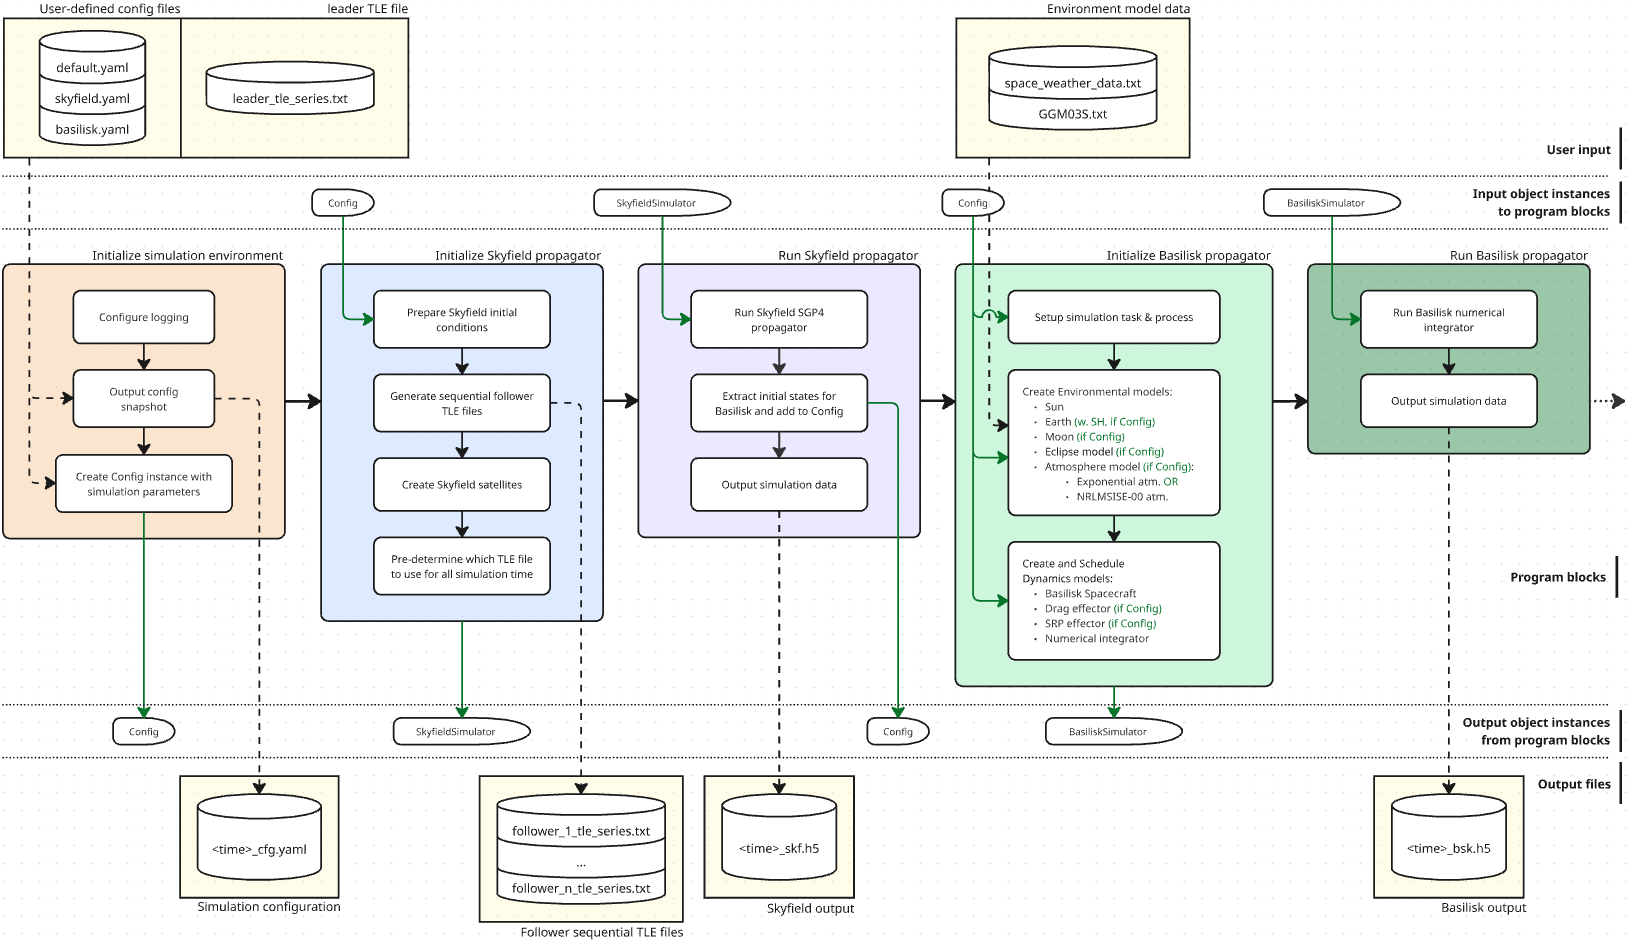
\includegraphics[width=1.0\textwidth]{Figures/04Method/Propagation Accuracy Comparison Simulator Flowchart.png}
    \caption{Adopted from \cite{hystad2025}}.
    \label{fig:propagator_comp_flow} 
\end{figure}


\section{Skyfield SGP4 Reference Methodology}
\begin{comment}
This section should present:
* TLE handling / follower generation
* Sequential TLE usage
* Why this is useful as a propagation comparison baseline
\end{comment}


\section{Propagation Initialization \& Execution}
\begin{comment}
Should present: (I am a bit unsure about this section => Subject to change. NOTE: Some of this might be better suited for the "Validation and Mission analysis methodology" chapter)
* The orbital configuration used (initial along-track spacing)
* Spacecraft configuration (reduced variant of the one presented earlier)
* Time horizon
\end{comment}


\cleardoublepage


\chapter{GNSS-R Formation Flight Simulator}
\label{chap:lifetime}
\begin{comment}
* Declare some sort or terminology when referring to each simulation run inside Monte Carlo:
    - One Monte Carlo (MC) run corresponds to multiple gnss-r formation flying simulations, or simply multiple simulation runs. 
    - Simulator is used to refer to the entire thing, which is the same as saying one MC run. 
\end{comment}


\section{Simulation Architecture}

\begin{figure}[H]
    \centering
    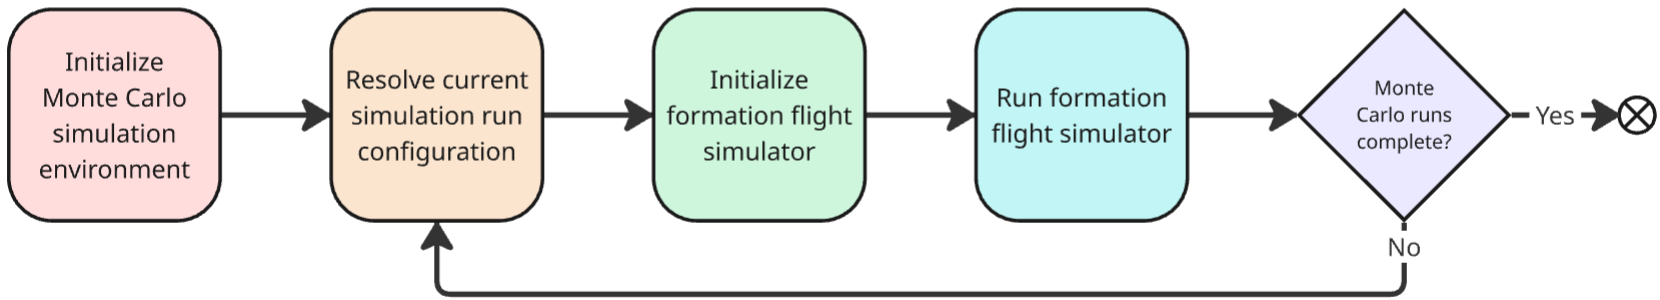
\includegraphics[width=0.8\textwidth]{Figures/04Method/Abstracted formation flight simulator.png}
    \caption{Simplified GNSS-R formation flight simulator flow diagram}.
    \label{fig:simple_formfly_flow} 
\end{figure}

The high-level execution flow of the GNSS-R Formation Flight Simulator is shown in Figure \ref{fig:simple_formfly_flow}. The simulator is organized into five main program blocks: initialization of the \gls{mc} simulation environment, resolution of the current simulation run configuration, initialization of the formation flight simulator, execution of the formation flight simulator, and evaluation of whether additional \gls{mc} runs remain. These blocks can be divided into two main parts, separated by the vertical dashed line in the detailed flowchart in Figure \ref{fig:formfly_flow}. The left part acts as a simulation run orchestrator, where the \gls{mc} environment is configured, and run-specific configuration files are prepared. The right part represents the iterative execution of individual simulation runs, where each run is initialized, executed, and written to file before the next queued run is started. As in the Comparative Propagation Simulator architecture presented in Section \ref{sec:propagator_architecture}, the detailed flowchart is divided into vertically stacked layers representing input files, internal object instances, program blocks, transferred output objects, and generated output files. However, unlike the Comparative Propagation Simulator, the GNSS-R Formation Flight Simulator does not include a separate Skyfield propagation module, but is built entirely around Basilisk numerical simulation.

\begin{figure}[H]
    \centering
    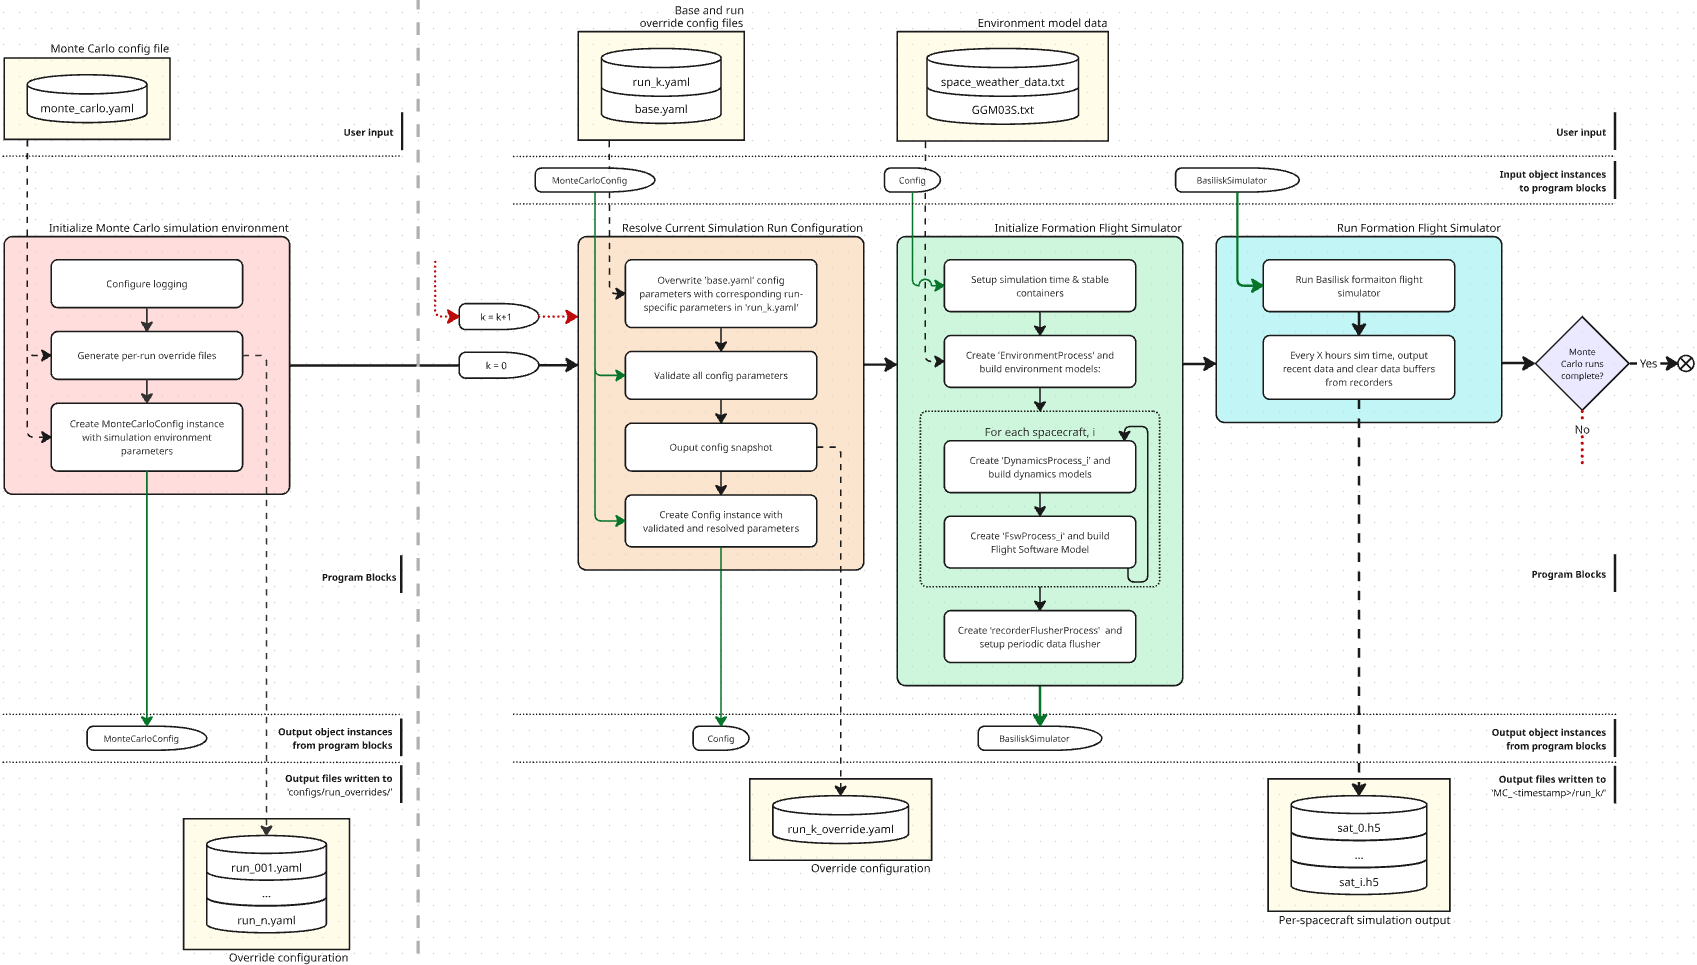
\includegraphics[width=1.0\textwidth]{Figures/04Method/Formation Flight Simulator.png}
    \caption{Detailed GNSS-R formation flight simulator flow diagram}.
    \label{fig:formfly_flow} 
\end{figure}

\subsection{Initialization of the Monte Carlo Environment}
The first program block initializes the \gls{mc} simulation environment from the user-defined configuration file \texttt{monte\_carlo.yaml}, and is considered the simulation run orchestrator. In this thesis, \gls{mc} execution is assumed to be enabled for all simulation cases, such that the simulator is structured around a queue of formation-flight simulation runs rather than a single isolated run. The \gls{mc} configuration defines the number of queued runs and the run-specific parameter variations used to generate override configuration files. If $n$ simulation runs are queued, $n-1$ override files are generated. Finally, the validated \gls{mc} settings are collected into a global \gls{mc} configuration instance, which is passed to the iterative part of the simulator and determines how the queued formation-flight simulations are executed.


\subsection{Current Run Configuration Resolution}
The next program block resolves the configuration for the current simulation run. This step is similar to the configuration initialization used in the Comparative Propagation Simulator, described in Section \ref{sec:propagator_init}, but is extended to support iterative \gls{mc} execution. For the first simulation run, the configuration is defined directly by the default scenario in \texttt{base.yaml}. For all subsequent runs, the corresponding override file \texttt{run\_k.yaml} is loaded and used to replace selected parameters in \texttt{base.yaml}, where $k$ denotes the current simulation run index. This allows each queued run to modify a limited set of scenario parameters while preserving the remaining default configuration. Once the current run configuration has been resolved, all parameters are validated and written to a timestamped configuration snapshot. As in the Comparative Propagation Simulator, this snapshot provides traceability by allowing each generated output data set to be linked to the exact parameter values used to produce it. Finally, the validated parameters are collected into a run-specific \texttt{Config} instance, which is passed to the formation flight simulator initialization block.


\subsection{}



\begin{comment}
This section should explain the high-level flow of the gnss-r formation flight simulator. It should contain the following:
* 1st paragraph:
    - Just like in the corresponding section for the other simulator, start by explaining the main modules aka. program blocks of the simulator, which is clearly shown in Figure \ref{fig:simple_formfly_flow} (the same program blocks is shown in \ref{fig:formfly_flow, but it is harder to make out})
        1. Setting up the Monte Carlo simulation environment
        2. Resolve current simulation run configuration
        3. Initialize formation flight simulator
        4. Run formation flight simulator
        5. Repeat from 2 if there are more simulations queued in the Monte Carlo run. 
    - The main modules can therefore be divided into two sections, which is divided by the vertical dotted line in the flowchart \ref{fig:formfly_flow}: the simulation run orchestrator on the left, and the iterative simulation runs on the right. 
    - The flowchart is also divided into different vertically stacked layers. Just like in Section \ref{sec:propagator_architectur}, the top and bottom layers represent the input and output files, the middle layer shows the program blocks, and the adjacent layers show how object instances are passed between them. Though, it is important to note that the left and right sections output files to different directories. 
    - Point out that, unlike the other simulator, the gnss-r formation flight simulator does not include its own skyfield module, but is entirely built upon the Basilisk framework. 

* 2nd paragraph (Initialization of the Monte Carlo environment)
    - The Monte Carlo (MC) initialization program block is responsible for defining the global Monte Carlo configuration from user input (\texttt{monte_carlo.yaml}).
    - After the \gls{mc} configuration file is loaded, it is used to generate n override configuration files, where n denotes the number of queued simulation runs-1.
    - Each override configuration file contain any number of parameters that override the default scenario, which enables the changing different scenario parameters between queued simulation runs.
    - Finally, the loaded monte carlo configuration file is used to create a global MonteCarloCondig.

* 3rd paragraph (Current run configuration resolution)
    - Explains how the "Resolve current simulation run configuration" program block works:
    - This is very similar to the initialization of the simulation environment program block described in Section \ref{sec:propagator_init}. The only substantial difference is that the iterative runs require resolving a combination of parameters from default.yaml, and run_k.yaml
    - This is the first step of this program block. For the very first simulation run, only the configuration parameters from \texttt{default.yaml} are used, but in every other following runs (k != 0), the parameters in run_k.yaml override the corresponding parameters in base.yaml. 
    - Then all resolved config parameters are validated, before a snapshot of the simulation configuration is exported. As mentioned before, this is important for traceability because it allows checking what parameters were used to generate an output data set at a later time. 
    - Finally, the validated parameters are  collected into a Config instance 


* 4th paragraph
    - Explains how the current run Basilisk GNSS-R formation flight simulator is initialized and run.
    - state that this high-level flow is very similar to "Basilisk Propagator Flow" presented in Section \ref{sec:basilisk_propagator_flow}


For later paragraphs: (avoid for now)
    Should be compared to the propagator simulator because this is an expansion/re-structured variant
    * Like in the Comparative propagation simulator "simulation architecture" section, this section should start by explaining the main program blocks by referencing the flow diagram \ref{fig:formfly_flow}. 
    * Task/process structure and resulting execution order
    * State that the old super-process has been split into environment and dynamics processes
    * Explain what each process is responsible for 
    * Conclude by saying that although this flowchart nicely presents the high-level simulator flow, it hides the inner complexity of the GNSS-R GNC modules. This will be explored in further detail in the coming sections. 

\end{comment}




\section{Electronic Power System}
\begin{comment}
Consumers and generators of electricity. How these effect battery, and how battery thresholds are defined. 
\end{comment}


\section{Flight Software}
\begin{comment}
* Overall structure, how is it all connected and run during execution
* Guidance pointing logic w. all states and mode transitions
* MRP feedback pointing controller 
* Formation control 
\end{comment}

\subsection{Software Architecture}

\subsection{Pointing Guidance Logic}

\subsection{MRP Feedback Pointing Controller}

\subsection{Formation Controller}

\section{Simulator inputs}

\begin{figure}[htbp]
    \small
    \dirtree{%
    .1 GNSS-R Formation Flight Simulator.
    .2 EnvironmentProcess.
    .3 EnvironmentTask.
    .4 spiceObj [20].
    .4 eclipseObj [20].
    .4 groundStation(s) [20].
    .4 atmObj [20].
    .3 MsisInputUpdaterTask.
    .4 msisInputUpdater [20].
    .2 DynamicsProcess\_\textless sat\_idx\textgreater.
    .3 DynamicsTask\_\textless sat\_idx\textgreater.
    .4 scObj.
    .4 dragEffector [20].
    .4 srpEffector [20] .
    .4 solarPanel(s) [20].
    .4 rwEffector [20].
    .4 thrusterEffector [20].
    .4 fuelTankEffector [20].
    .4 battery [20].
    .4 obcPowerSink [20].
    .4 rwPower(s) [20].
    .4 thrusterStateRecorder [10].
    .4 fuelTankStateRecorder [10].
    .4 rwStateRecorder(s) [10].
    .4 rwStateRecorder(s) [10].
    .4 batteryStateRecorder [10].
    .4 obcPowerSinkRecorder [10].
    .4 solarPanelPowerRecorders(s) [10].
    .2 FswProcess\_\textless sat\_idx\textgreater.
    .3 FswTask\_\textless sat\_idx\textgreater.
    .4 scheduler [20].
    .4 navTransRecorder [10].
    .4 navAttRecorder [10].
    .4 attRefRecorder [10].
    .4 attErrRecorder [10].
    .4 cmdTorqueRecorder [10].
    .4 rwMotorTorqueRecorder [10].
    .2 RecorderFlusherProcess.
    .3 RecorderFlusherTask [20].
    .4 recorderFlusher [20].
    }
    \caption{Hierarchical process-task-model structure of the GNSS-R formation flight Basilisk simulator. The number in square brackets denote the model priority, where higher priority models are updated first. Same-priority tasks are orderly updated from the top-down within a task. ''\textit{<sat\_idx>}'' represent per-spacecraft processes and tasks.}
    \label{fig:basilisk_simulator_hierarchy}
\end{figure}

\cleardoublepage


\chapter{Shared Simulator Configuration}
\label{chap:shared}
% Introduction should introduce the two distinct simulators, and then state that they use some common physical modeling. Also state that these models are confined to the Basilisk framework



\section{Shared Spacecraft Configuration}
\begin{comment}
Present the full spacecraft configuration we're talking:
* geometry and body frame definition
* RW
* Thruster
* Fuel tank
* EPS with all its components
* antennas
* Combined mass (dry and wet)
* Estimated inertia

Also state that all EPS, ADCS and propulsion subsystem dynamics are disabled for the comparative propagator. 
\end{comment}


\section{Shared Orbital Environment Models}
\begin{comment}
State all environment models used inside the Basilisk simulators:
* Earth with spherical harmonics
* 3rd body pull from Sun and Mood
* SRP
* Drag (exp and MSIS)

Also state that the propagator simulator implements toggling of any combination of environment models in order to isolate their effects. 
\end{comment}



\section{Shared Numerical Integration Configuration}
\begin{comment}
State the numerical integrator configuration:
* Integrator
* Timestep

With reasoning. Mention results from specialization project and instability constraints. 
\end{comment}
\cleardoublepage


\chapter{Mission Analysis Methodology}
\label{chap:experiments}
\section{Propagation Validation Methodology}
\begin{comment}

\end{comment}


\section{GNSS-R Mission Analysis Methodology}
\begin{comment}

\end{comment}

\subsection{Mission Lifetime Definition}

\subsection{Evaluation Metrics}

\subsection{Monte Carlo \& Scenarios}
\cleardoublepage


\chapter{Results}
\label{chap:results}
% \section{Results overview and roadmap}

Plotting ideas for part 2:
\begin{itemize}
    \item The big important plot: Fuel level over time
    \item It would be interesting to see natural formation drift, and calculate delta-V requirements to compensate for this drift to estimate lifetime. This estimate could be used to validate results.
    \item Show the relative differences in applied perturbation acceleration from differential J2 and drag to explain drift rate
    \item Each subsystem should be validated in addition to showing the full fuel consumption over simulation duration:
    \begin{itemize}
        \item RW speed/torque step response
        \item Thruster force output as a function of fuel level (/tank pressure)
        \item MRP feedback controller tracking error and/or step response (would also be interesting to see a step response for different fuel levels)
        \item Decomposed net power and battery level (should also show the illumination factor in the same/adjacent plot and the FSW state)
    \end{itemize}
\end{itemize}

\section{Bsk Skf comparison}
State clearly that all differences are computed as Basilisk minus Skyfield.


\subsection{Overall Earth-relative Divergence}

\begin{figure}[H]
    \centering
    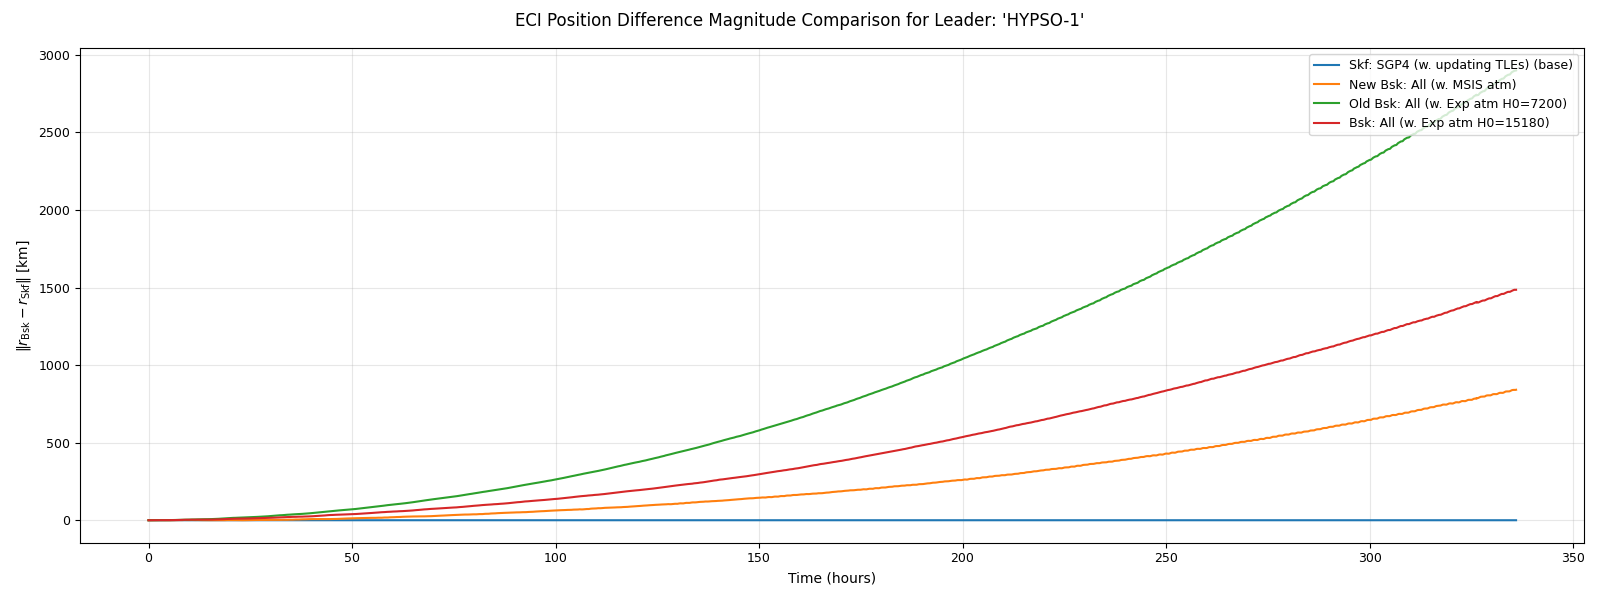
\includegraphics[width=0.6\textwidth]{Figures/05Results/bsk_skf_comparison/Ex1 - ECI pos difference magnitude.png}
    \caption{ECI position difference}
    \label{fig:1} 
\end{figure}

\begin{figure}[H]
    \centering
    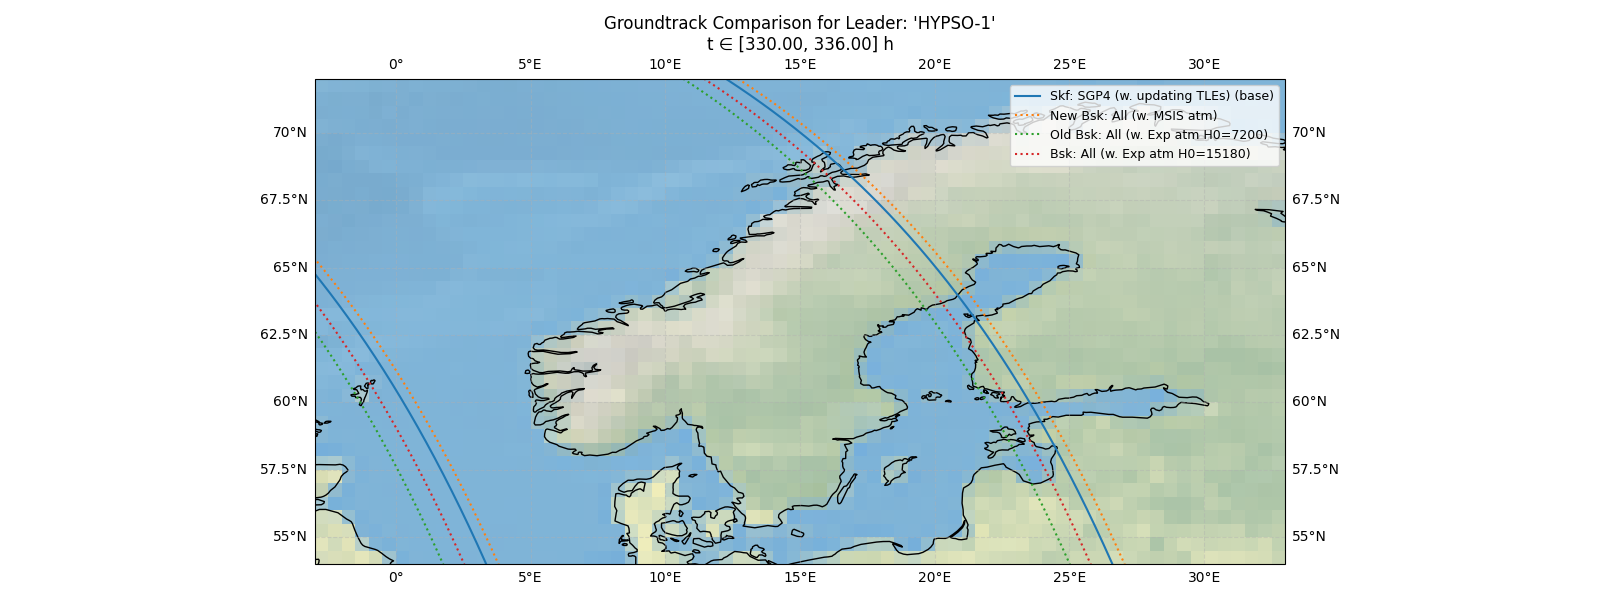
\includegraphics[width=0.6\textwidth]{Figures/05Results/bsk_skf_comparison/Ex1 - Groundtrack comparison.png}
    \caption{}
    \label{fig:2} 
\end{figure}



\subsection{Decomposition of Position Error in RTN Frame}

\begin{figure}[H]
    \centering
    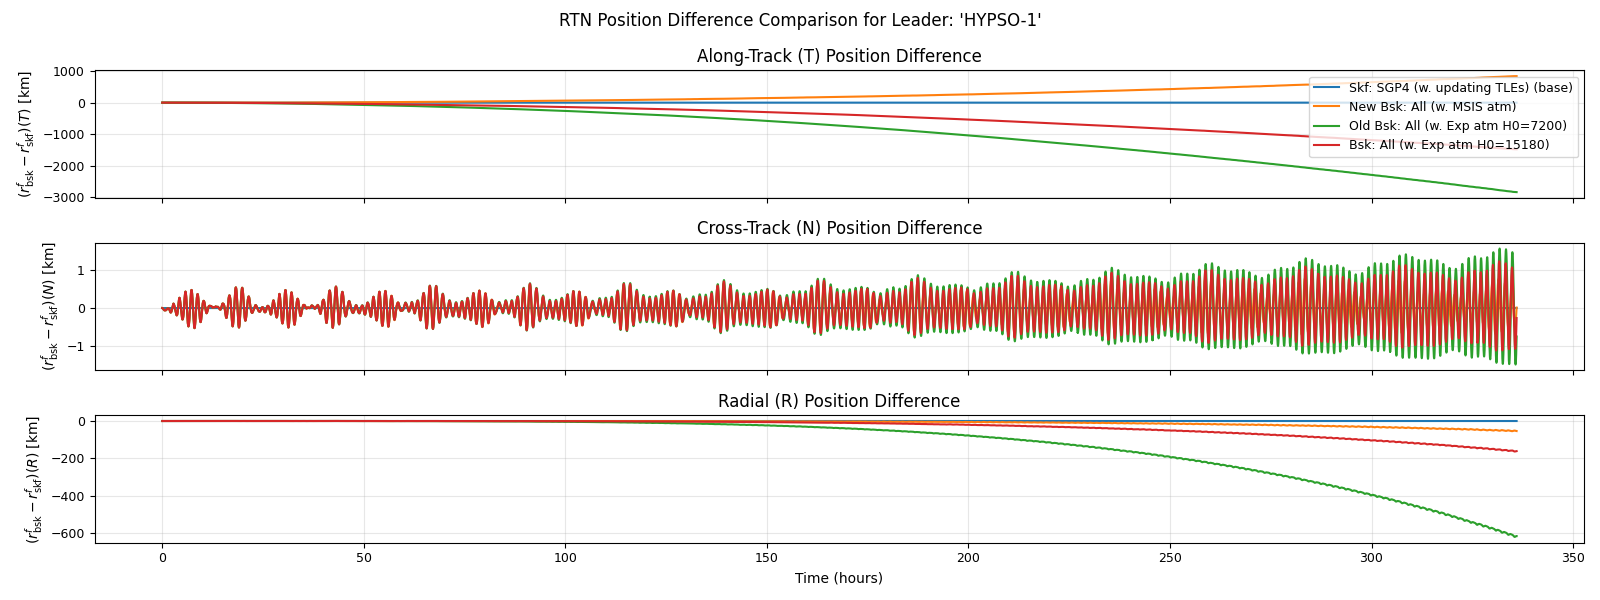
\includegraphics[width=0.6\textwidth]{Figures/05Results/bsk_skf_comparison/Ex1 - RTN pos difference.png}
    \caption{}
    \label{fig:3} 
\end{figure}



\subsection{Altitude Difference Comparison}

\begin{figure}[H]
    \centering
    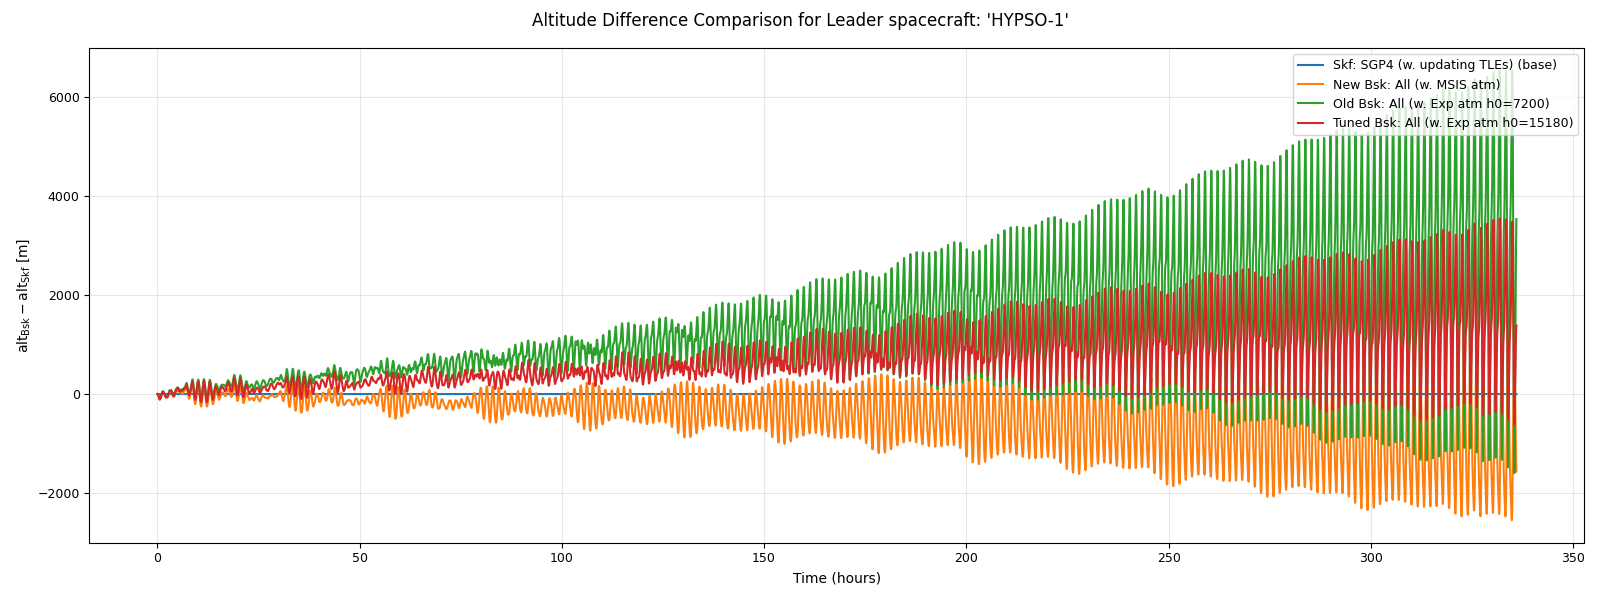
\includegraphics[width=0.6\textwidth]{Figures/05Results/bsk_skf_comparison/Ex1 - Altitude difference.png}
    \caption{}
    \label{fig:4} 
\end{figure}
\hl{I might try to remove some oscillations through data processing to highlight the trends and remove the altitude difference caused by different positions in the along-track and cross-track directions. Remove the }


\subsection{Orbital Element Drift}

\begin{figure}[H]
    \centering
    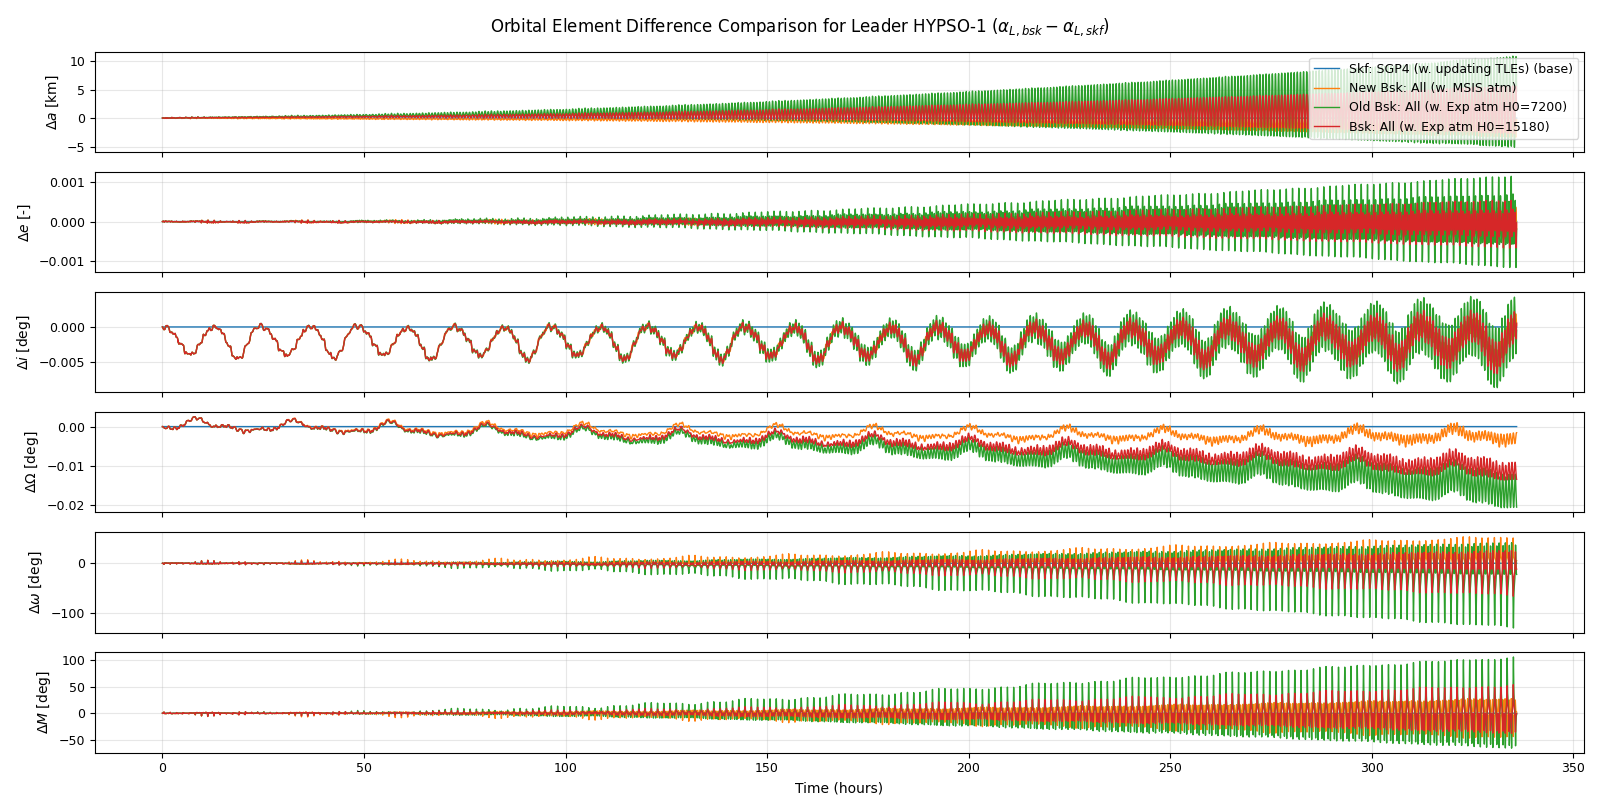
\includegraphics[width=0.6\textwidth]{Figures/05Results/bsk_skf_comparison/Ex1 - OE difference comparison.png}
    \caption{}
    \label{fig:5} 
\end{figure}

% \begin{figure}[H]
%     \centering
%     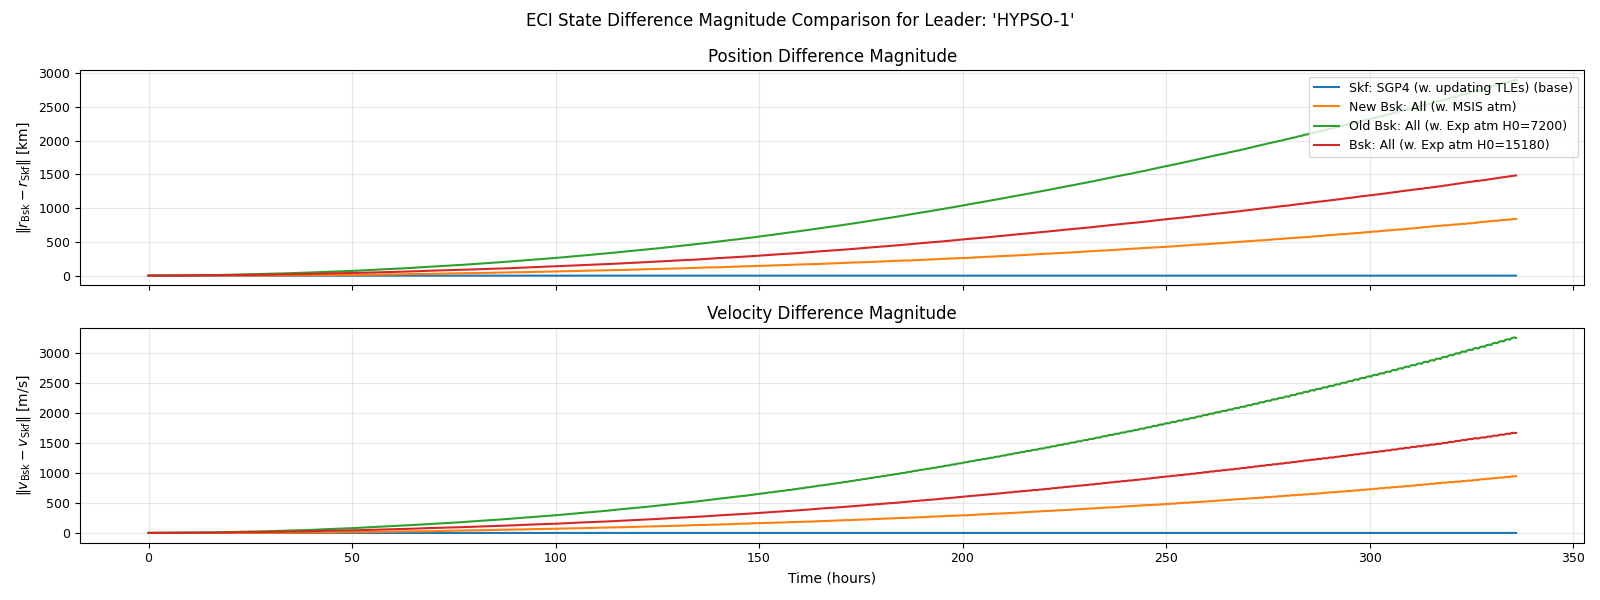
\includegraphics[width=0.6\textwidth]{Figures/05Results/bsk_skf_comparison/Ex1 - ECI pos-vel difference magnitude.png}
%     \caption{}
%     \label{fig:6} 
% \end{figure}


\subsection{Propagator Comparison Summary}

\begin{figure}[H]
    \centering
    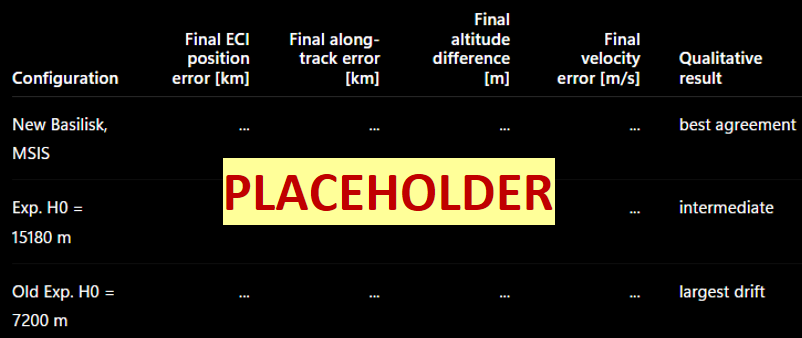
\includegraphics[width=0.6\textwidth]{Figures/05Results/bsk_skf_comparison/Bsk-Skf comparison summary table.png}
    \caption{Basilisk/Skyfield-SGP4 comparison summary}.
    \label{fig:bsk_skf_summary} 
\end{figure}








% ======================================================================================================================================= %
% ======================= G N S S - R    F O R M A T I O N    F L I G H T    S I M U L A T O R    R E S U L T S ======================= %
% ======================================================================================================================================= %


\section{Deployment Velocity Formation Acquisition Fuel Sensitivity}
\begin{comment}
This builds heavily on how "Formation Acquisition" is defined in the methodology

Data analysis that needs to be performed:

01. For each run, compute $t_{acq}$ and $m_{acq} = m_{fuel}(0) - m_{fuel}(t_{acq})$

02. For each run, compute the accumulated fuel consumption. This will enable other analyses and make comparisons simpler and more intuitive

Results that will be presented:


CORE PLOTS FOR THE DEPLOYMENT SENSITIVITY RESULT

1. Follower fuel consumption from all runs in one plot
    x-axis: time [h]
    y-axis: cumulative follower fuel consumed [g]
    one curve per deployment-speed case
    vertical marker at t_acq for each run, if acquired

2. Accumulated acquisition fuel consumption as a function of differential deployment speed
    x-axis: differential deployment speed magnitude [m/s]
    y-axis: acquisition fuel consumption [g]

3. Acquisition time as a function of differential deployment speed
    x-axis: differential deployment speed magnitude [m/s]
    y-axis: acquisition time [h]
4.1 RTN leader-follower relative position 3D trajectory for a selected set of runs
    RTN components in space
    choose subset of runs (0, 2, 4 diff speed)
4.2 RTN leader-follower relative positions decomposed for a selected set of runs
    choose subset of runs (0, 2, 4 diff speed)
    x-axis: time [h]
    y-axis: R, T, N components [m]
    horizontal lines for in-formation R, T, N upper/lower limit




SUPPORTING PLOTS FOR BURN Behavior 

5. Dual-bar plot showing acquisition accumulated thrust on-time and number of burns for each differential deployment speed
    x-axis: differential deployment speed magnitude [m/s]
    y-axis (left, corresponding to left vertical bar): acquisition accumulated thruster on-time / avg. thruster on-time
    y-axis (right, corresponding to right vertical bar): number of burns completed during acquisition


FEASIBILITY CHECKS

6. Operational mode timeline for all deployment cases / Another option is to show table with accumulated time spent in each mode for each run
    x-axis: time [h]
    y-axis: operational mode for each run
    show vertical lines for each run t_{acq}

7. Table summarizing some feasibility/accuracy metrics for each run:
    * The average attitude tracking error during burns [deg]
    * The accumulated time when burns were not possible (because of emergency mode)


SUMMARY TABLE

8. Show the following fields for every run:
    * Leader/follower deployment speed [m/s]
    * Differential speed [m/s]
    * Acquired?
    * Acquisition time [h]
    * Acquisition fuel [g]
    * Burns before acquisition
    * Avg. thruster on-time
    * Max RTN error [m]
    * Avg. attitude tracking error during burn
    * Min battery [%]



\begin{figure}[H]
    \centering
    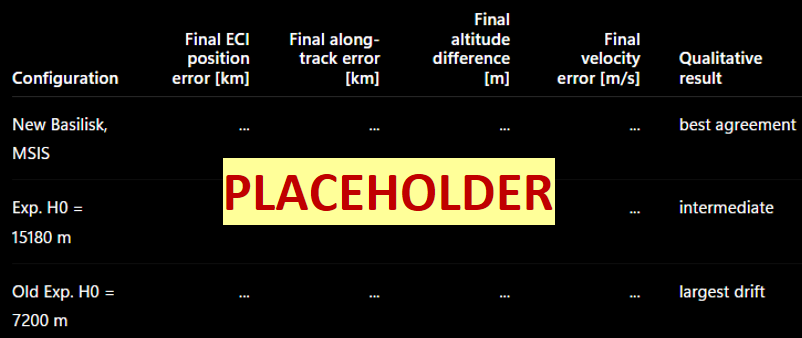
\includegraphics[width=0.6\textwidth]{Figures/05Results/bsk_skf_comparison/Bsk-Skf comparison summary table.png}
    \caption{Basilisk/Skyfield-SGP4 comparison summary}.
    \label{fig:bsk_skf_summary} 
\end{figure}



\end{comment}


\section{Steady-State Formation Maintenance Fuel Rate Estimation}
\begin{comment}


Supporting plot: 
Show the average pointing error during burns 


\end{comment}


\section{GNSS-R Formation Flight Lifetime Estimation}
\cleardoublepage


\chapter{Discussion}
% \subsection{comparative bsk / sgp4 propagation}
% * TLEs are tied to real spacecraft, which mean that their change in orbit over time is the result of real perturbations acting on the real spacecraft. HYPSO-1, which is the corresponding satellite for the TLEs used by the Skyfield SGP4 models, is an Earth-observation satellite with a fixed imaging payload. This means its attitude will change over time to 
% * TLEs are estimated from observations, which mean there are intrinsic parameter uncertanties.


% \subsection{deployment velocity acquisition fuel consumption}
% % * The formation appears to be a bounded periodic relative orbit with CPO-like characteristics. The larger along-track amplitude is expected for HCW-type relative orbital motion and does not by itself mean the formation is not a CPO.
% % * I am a little careful not to make too hard claims here since I don't really know different formation types that well: 
% %     Limited to a 2 spacecraft concentric formation due to formation-maintenance implementation constraints. This is because the formation targets a classic orbital element difference setpoint, which cannot be used to achieve a precise constant-separation or circular projected orbit formation discussed in \cite{hill2025hydroswarm}.


% \subsection{Steady-state fuel consumption}
% * The corresponding campagin was not run at the full 60-day duration as planned, but ended prematurely at 24 days due to memory overflow issues in the GNSS-R Formation Flight Simulator. 


% \section{GNSS-R Formation Flight Lifetime Estimate}
% * comment on the fact that the linear fitted m\_acq is negative for the zero differential deployment speed case. 
\hl{Introduction}

\section{Propagation Benchmark Interpretation}
\begin{comment}
* 
\end{comment}

\subsection{Basilisk-Skyfield-SGP4 Divergence Interpretation}

Across the same-spacecraft comparison results, the primary thesis Basilisk configuration shows the smallest divergence from the continuously updating Skyfield-SGP4 baseline. Figure \ref{fig:same_sc_ECI_state_mag_diff} shows that the specialization-project exponential atmosphere configuration reaches approximately three times the position difference of the primary thesis configuration after the 14-day propagation interval, while the re-tuned exponential atmosphere configuration reaches approximately 1.5 times the position difference. Since the main difference between the evaluated Basilisk configurations is the atmospheric density model, the observed ordering can be interpreted primarily through the different drag environments experienced by the spacecraft.

The altitude difference in Figure \ref{fig:same_sc_altitude_difference} supports this interpretation. The primary thesis configuration with the NRLMSISE-00 atmosphere model gradually drops below the Skyfield-SGP4 reference altitude, while both exponential atmosphere configurations drift toward higher relative mean altitude. This indicates that the primary thesis configuration experiences stronger effective drag than the exponential atmosphere configurations over the comparison interval. The re-tuned exponential atmosphere model reduces the altitude divergence relative to the specialization-project configuration, but it does not reproduce the same altitude evolution as the NRLMSISE-00 configuration.

The RTN decomposition in Figure \ref{fig:same_sc_pos_RTN_decomposition} shows that the resulting same-spacecraft position difference is dominated by radial and along-track drift. Because we are effectively considering the relative drift between two deactivated spacecraft affected by different amounts of drag, the relative drift mechanics covered in Section \ref{sec:diff_perturb} apply. Sustained differential drag will accumulate into substantial along-track drift. This is because a sustained altitude difference changes the relative orbital period, which accumulates into along-track separation over time. The exponential atmosphere configurations maintain a higher relative mean altitude than the Skyfield-SGP4 baseline and therefore increasingly lag behind the reference trajectory. This produces the negative along-track difference observed in the RTN decomposition. In contrast, the primary thesis configuration drops to a lower relative mean altitude, corresponding to a shorter relative orbital period, and therefore drifts ahead of the Skyfield-SGP4 baseline in the positive along-track direction.

The radial component in Figure \ref{fig:same_sc_pos_RTN_decomposition} should be interpreted together with the dominant along-track separation. Since the RTN frame is defined at the Skyfield-SGP4 leader position, the radial component represents the direction along its position vector away from the Earth. For large along-track separations, this radial projection is not equivalent to the altitude difference, but rather the circular curvature of the orbit. Thus, a sufficiently large along-track difference correspond to a negative radial deviation for spacecraft in the same approximate near-circular orbit.

The same differential-drag interpretation also applies to the same-formation drift difference shown in Figure \ref{fig:same_form_drift_RTN_decomposition}. All Basilisk configurations predict a larger leader-follower along-track drift than the Skyfield-SGP4 baseline. However, the ordering between the Basilisk configurations is reversed and less separated compared to the same-satellite state comparison. The primary thesis configuration gives a slightly larger same-formation along-track drift difference, while the exponential configurations remain close to it. This indicates that the atmospheric model has a much stronger effect on the absolute Earth-relative propagation of each spacecraft than on the passive leader-follower drift over the same interval. The primary thesis configuration likely diverges more than the others, because its differential drag drift is stronger due to each spacecraft being subject to higher intensity drag. Also, the very small relative divergence between the Basilisk configurations are probably due to the \gls{eci}-fixed spacecraft attitude assumption, where the difference in incident flow in each body-fixed frame are only slightly different due to the initial $1^\circ$ in-plane separation angle. 

\begin{comment}
Discuss around the fact that the thesis propagator configuration has the least divergence across all same-spacecraft difference representation:
    * Across all same-spacecraft comparisons of various Basilisk configurations against the updating-TLE Skyfield-SGP4 comparison baseline, the primary thesis configuration show significantly less divergence than all other Basilisk configurations. Figure \ref{fig:same_sc_ECI_state_mag_diff} show that the divergence distance for the specialization-project untuned exponential atmosphere is approximately three times that of the primary thesis NRLMSISE-00 configuration after a 14-day propagation duration. The tuned exponential atmosphere configuration deviation distance is approximately 1.5 times after the same propagation duration. 
    * Since the only difference between the Basilisk configurations are their respective atmosphere models, it is natural to evaluate the deviations in terms of differences in experienced drag. 
    * Figure \ref{fig:same_sc_altitude_difference} showing the altitude same-satellite differences offers important insight. Here, the primary thesis configuration's mean altitude slightly drops below the reference Skyfield-SGP4 altitude, while the tuned and old Basilisk configurations have increasingly higher relative mean altitudes. This strongly indicates that the primary thesis configuration with its NRLMSISE-00 atmosphere model is subject to more drag than the exponential atmosphere counterparts. 
    * Because we are effectively considering the relative drift between two deactivated (no formation control) satellites affected by different amounts of drag, the relative drift mechanics covered in Section \ref{sec:diff_perturb} apply. Sustained differential drag will accumulate into substantial along-track drift, which is exactly what the RTN component divergence shows in Figure \ref{fig:same_sc_pos_RTN_decomposition}. 
    * This is because The drag-induced relative gain in mean altitude for the tuned and specialization-project Basilisk configurations mean that their relative orbital period is extended, which cause them to increasingly lag behind the Skyfield-SGP4 baseline. 
    * The opposite is true for the primary thesis configuration, where more drag causes its mean relative altitude to decrease, which decreases its relative orbital period. This in turn causes this satellite to lead in front of the Skyfield-SGP4 baseline, thus explaining the positive divergence in the along-track direction. 
    * The radial divergence is a consequence of the along-track separation. Because the radial direction is defined along the Skyfield-SGP4 leader's position vector, any along-track same-satellite position difference in the same orbital plane will manifest as a negative radial deviation. 
    
Same-formation position drift difference:
    * The same differential drag argument can be used to explain the observed divergence in the same-formation position drift differences shown in Figure \ref{fig:same_form_drift_RTN_decomposition}. Here, all configurations give a larger along-track leader-follower position drift than the Skyfield-SGP4 baseline, and the previous divergence order has reversed. The primary thesis configuration likely diverges more than the others, because its differential drag drift is stronger due to each spacecraft being subject to higher intensity drag. Also, the very small relative divergence between the Basilisk configurations are probably due to the \gls{eci}-fixed spacecraft attitude assumption, where the difference in incident flow in each body-fixed frame are only slightly different. 

\end{comment}


\subsection{Updating-TLE SGP4 as a Comparison Baseline}

The interpretation of the comparative propagation results depends on the quality of the continuously updating Skyfield-SGP4 baseline. This baseline is not a true physical ground truth, but an observation-updated reference generated from a sequence of \glspl{tle}. Since the propagated \gls{tle} is replaced regularly throughout the comparison interval, the SGP4 prediction error is not allowed to accumulate over the full 14-day horizon in the same way as it would for a static-\gls{tle} propagation. This makes the updating-\gls{tle} baseline a more useful long-horizon comparison reference than the single-\gls{tle} baseline used in the specialization project~\cite{hystad2025}.

The frequent \gls{tle} updates also explain why no distinct correction discontinuities are visible in the comparison figures. Over short propagation intervals, SGP4 is generally expected to remain sufficiently close to the estimated spacecraft state that the transition between adjacent \glspl{tle} does not dominate the plotted state histories. The resulting baseline is therefore best interpreted as a sequence of short SGP4 predictions tied together by updated orbit estimates, rather than as one uninterrupted long-horizon physical propagation.

However, the \glspl{tle} used by the Skyfield-SGP4 baseline are tied to the real HYPSO-1 spacecraft. The orbital evolution represented by the \gls{tle} sequence therefore includes the effect of real perturbations acting on HYPSO-1, including effects associated with its actual attitude and operational history. Since HYPSO-1 is an Earth-observation satellite with a body-fixed imaging payload, its attitude may vary over time due to science objectives. This means that the effective drag experienced by the real spacecraft may differ from the drag experienced by the simplified Basilisk spacecraft, which is propagated with a fixed attitude in the comparative propagation analysis. As a result, differences between Basilisk and the updating-\gls{tle} Skyfield-SGP4 would still be present with a perfect atmosphere model simply because of different experienced attitude-coupled drag.

The updating-\gls{tle} Skyfield-SGP4 trajectory is therefore a valuable comparison baseline, but it should not be interpreted as exact truth. It provides a practical reference for evaluating whether the primary thesis Basilisk configuration improves over the specialization-project configuration and for quantifying the scale of the remaining propagation divergence. The comparison result should consequently be interpreted as agreement with an observation-updated SGP4 reference, rather than as an absolute validation of the Basilisk propagator.
\begin{comment}
    * The evaluation of the primary thesis Basilisk configuration propagation accuracy depends on the accuracy of the comparative model, the updating-TLE Skyfield-SGP4.
    * Because the TLEs are updated every few hours, its prediction accuracy is again dependent on the TLEs, and its physical interpretation. 
    * One thing to point is that although the TLEs are frequently updated, no visible corrections are visible in the propagator comparison figures. This is because the SGP4 TLE propagation algorithm is widely known to be sufficiently accurate for 1-2 days before noticeably deviation from the real state, depending on the orbit and TLE estimation accuracy. Thus, the SGP4 propagation error does not have enough time to accumulate before the propagated TLE is updated.
    * However, the TLEs are tied to real spacecraft, which mean that their change in orbit over time is the result of real perturbations acting on the spacecraft. HYPSO-1, whose TLEs are used in all the Skyfield-SGP4 propagator, is an Earth-observation satellite with a fixed imaging payload. This means its attitude will change over time to perform science operations, causing its experienced drag to vary with time.
    * This means that, even with a perfect Basilisk atmosphere model, deviations will still appear if their attitudes are  different over time. 
    * Still, because the updating TLEs guarantee that the state error of the comparison baseline is small, it still a valuable comparison baseline, and an improvement from the static-TLE baseline considered in the specialization project in \cite{hystad2025}
\end{comment}



\subsection{Implications for the Lifetime Analysis}
\label{sec:comparison_implication_for_lifetime}

The comparative propagation analysis indicates that the primary thesis Basilisk configuration is the most accurate of the evaluated Basilisk configurations relative to the continuously updating Skyfield-SGP4 baseline. Across the same-spacecraft state comparisons, the NRLMSISE-00 configuration produces substantially smaller divergence than both exponential-atmosphere configurations. This supports the use of the primary thesis configuration as the propagation environment for the GNSS-R formation flight lifetime analysis. However, the primary thesis configuration still accumulates a significant same-satellite difference over the 14-day comparison interval, dominated by radial and along-track drift. 

Perhaps more importantly for the lifetime analysis, is the same-formation position drift difference. Although the major drift difference between the primary thesis configuration and the Skyfield-SGP4 baseline remain unexplained, the increased along-track formation drift will require additional formation-maintenance maneuvers. The resulting lifetime estimations will therefore likely be pessimistic in its predictions. However, the updating-TLE Skyfield-SGP4 baseline also limits how strongly the propagation comparison can be interpreted. Since the baseline is an observation-updated SGP4 reference rather than a precise orbit-determination truth model, the observed Basilisk-Skyfield differences are not direct physical prediction errors. The comparison still provides useful evidence that the thesis configuration improves over the specialization-project configuration, but it does not fully validate the long-horizon Basilisk trajectory.









\section{Formation Fuel Consumption}

\subsection{Acquisition Consumption}
\label{sec:discussion_acq_consumption}

The deployment sensitivity results show summarized in Figure \ref{fig:diff_deploy_curve_fitting}, show that acquisition time is generally positively correlated with differential deployment speed, but that the relationship is not strictly increasing. The most visible exception is the $\Delta v_{\mathrm{dep}}=3.5~\mathrm{m/s}$ case, which acquired the formation after $3.92~\mathrm{h}$, compared with $5.48~\mathrm{h}$ for the $\Delta v_{\mathrm{dep}}=3.0~\mathrm{m/s}$ case and $5.43~\mathrm{h}$ for the $\Delta v_{\mathrm{dep}}=4.0~\mathrm{m/s}$ case. Since $t_{\mathrm{acq}}$ is determined directly from the \gls{oed} tolerance and dwell-time criterion, this non-monotonic behavior indicates that the selected acquisition criterion does not provide a perfectly smooth measure of the acquisition transient across the tested deployment cases.

The \gls{oed} histories shown in Figure \ref{fig:diff_deploy_oed} suggest that the acquisition criterion may be somewhat relaxed for the purpose of distinguishing the end of acquisition from the beginning of maintenance. For example, the $\Delta v_{\mathrm{dep}}=4.0~\mathrm{m/s}$ case performs several additional burns after its acquisition time, which further reduces the semi-major-axis difference toward the center of the tolerance band. Similarly, the eccentricity difference is not fully synchronized across all deployment cases until approximately $7.6~\mathrm{h}$, which is later than the largest recorded acquisition time. The cumulative fuel-consumption time series in Figure \ref{fig:diff_deploy_cum_fuel_consumption} also show several post-acquisition burn events of non-negligible size. These observations suggest that the exact numerical value of $t_{\mathrm{acq}}$ is sensitive to the selected \gls{oed} tolerances and dwell time, although the plots alone do not provide a strict separation between late acquisition burns and early maintenance burns.

The acquisition fuel consumption shows a more uniform dependence on differential deployment speed than the acquisition time. The only from this strictly increasing behavior is in the change from $\Delta v_{\mathrm{dep}}=0.0~\mathrm{m/s}$ to $\Delta v_{\mathrm{dep}}=0.5~\mathrm{m/s}$, where the measured acquisition fuel consumption decreases with differential deployment speed. The slightly lower acquisition fuel consumption for the $0.5~\mathrm{m/s}$ case may indicate that a small non-zero differential deployment speed can reduce the fuel needed to initiate the concentric formation. This makes sense considering this removes the need for an initial burn to separate the leader and follower spacecraft. For the remaining cases, the increasing trend is consistent with the larger velocity correction required to remove the initial deployment-induced relative motion and insert the follower into the target formation.

Because the acquisition time is on the order of a couple of hours for the cases studied in this thesis, the time-horizon is too short for any small differential orbital perturbations to take any noticeable effect, and cannot be considered a major driver for acquisition fuel consumption. Thus, the main driver of acquisition fuel consumption is the initial differential deployment condition and the corrective burns required to reach the desired formation. Modeling this cumulative fuel consumption purely as a function of $\Delta v_{\mathrm{dep}}$ is therefore a reasonable simplification. However, as discussed initially, the largest uncertainty in the extracted acquisition fuel values is likely associated with the acquisition-time definition itself, since changing the \gls{oed} tolerances or dwell-time requirement would shift the point at which cumulative fuel consumption is sampled. 

\begin{comment}
* Discuss the acquisition times. Are all transients gone at this point? Are the OED tolerances correctly tuned?
    - As presented in Figure \ref{fig:diff_deploy_curve_fitting}, the acquisition time is positivly correlated with the differential deployment speed. 
    - however, this relationship is not strictly increasing. The most extreme simulated case for this is the 3.5m/s deployment case which had 3.92hours acquisition time, compared to 5.48 for the 3m/s differential deployment case. This is comparable to the 1.5 and 2 m/s cases with 3.88 hours each. The 3.0m/s case also had the highest acquisition time of all cases, even higher than the highest differential deployment speed case at 5.43 hours. 
    - Since the acquisition time is directly determined by the \gls{oed} tolerances, this effect might be explained by too relaxed parameters. Evidence for this is present in Figure \ref{diff_deploy_oed}, where, for example, the 4m/s case performs several additional burns in order to change its semimajor axis closer to the center of the tolerances after its acquisition time. Additionally, we also see that the eccentricity difference is not fully synchronized for all cases until approximately 7.6 hours, which is greater than the highest acquisition time. 
    - This claim of too loose \gls{oed} tolerances is supported by Figure \ref{fig:diff_deploy_cum_fuel_consumption} that show multiple instances of many relatively large burns after the initial acquisition. However, this is not definitive proof as it is hard to distinguish between formation acquisition and maintenance burns by looking at the cumulative fuel consumption


Discuss the simulated acquisition fuel consumption: 
    * The acquisition fuel consumption trend shown, however, is more uniform. 
    * The only case of non-strict increase in acquisition time is in cases 0.0 (5.6g) to 0.5 m/s (5.39) diff deploy speed. 
    * This result is particularly interesting, because it suggests that it is less fuel intensive to achieve a formation with some non-zero differential deployment speed. This makes sense because it removes the need for the follower to expend fuel to accelerate to away from the leader before it can begin the insertion burns for the concentric formation. 
    * Otherwise, it makes sense that the for the acquisition fuel consumption to be strongly positively correlated with the differential deployment speed, because the follower spacecraft has to expend more fuel to correct for a higher the initial differential deployment speed.  



* What are the drivers for acquisition fuel consumption? (Is it reasonable to model acquisition consumption as a function of only $\Delta v_{\mathrm{dep}}$)
    * Because the acquisition time is on the order of a couple of hours for the cases studied in this thesis, the time-horizon is too short for any small differential orbital perturbations to take any noticeable effect, and cannot be considered a major driver for acquisition fuel consumption. 
    * Therefore, I would argue that modeling the acquisition fuel consumption purely as a function of $\Delta v_{\mathrm{dep}}$ is a fair assumption
    * However, because moving the acquisition time also changes the amount of cumulated consumed fuel before this time, the formation tolerances are probably the greatest source of uncertainty for acquisition fuel consumption. 
\end{comment}


\subsection{Steady-State Maintenance Consumption}
\label{sec:discussion_steady_state_fuel_consumption}

The steady-state fuel consumption result in Figure \ref{fig:steady_state_cum_consumption} show that the steady-state cumulative fuel consumption rate is not perfectly constant, but appears to decrease slightly over the 24-day simulation. This trend is physically reasonable, since a lower remaining propellant mass reduces the spacecraft mass, such that a given orbital correction requires slightly less thrust impulse, assuming that the required formation-maintenance corrections remain approximately the same. This behavior differs from the acquisition phase, where fuel consumption is dominated by a short sequence of corrective burns shortly after deployment. Regardless of how the acquisition time is defined, the deployment sensitivity fuel time series in Figure \ref{fig:diff_deploy_cum_fuel_consumption} clearly show that the burn frequency is strongly reduced after the initial formation insertion period. The remaining fuel consumption is therefore associated with slower formation-maintenance corrections, rather than the removal of the initial deployment-induced relative motion.

This behavior differs from the acquisition phase, where fuel consumption is dominated by a short sequence of corrective burns shortly after deployment. Regardless of how the acquisition time is defined, the deployment sensitivity fuel time series in Figure \ref{fig:diff_deploy_cum_fuel_consumption} clearly show that the burn frequency is strongly reduced after the initial formation insertion period. The remaining fuel consumption is therefore associated with slower formation-maintenance corrections, rather than the removal of the initial deployment-induced relative motion.

The steady-state drift mechanism is not expected to be dominated by large ballistic-coefficient differences between the spacecraft. As described in Section \ref{sec:diff_drag}, the differential atmospheric drag depends on differences in ballistic coefficient, which is affected by the drag coefficient and flow-normal cross-sectional area. In the simulated formation, both spacecraft use the same drag coefficient, and Figure \ref{fig:steady_state_eps_modes_final_day} shows that the leader and follower are synchronized in their operational modes during steady-state operation. Since the operational modes determine the attitude profile, the two spacecraft therefore spend most of the time in similar attitudes. This reduces differences in flow-normal area and gives the leader and follower very similar ballistic coefficients.

Some differential drag is still present because the follower follows an oscillatory relative trajectory around the leader. The radial component in Figure \ref{fig:diff_deploy_rtn_relative_position_decomposition} has an amplitude of approximately $400~\mathrm{m}$, which for small separation distances, correspond to a small periodic altitude difference between the leader and follower. The follower therefore periodically occupies slightly higher and lower atmospheric density regions than the leader. However, this separation is small compared with the orbital altitude, and the formation controller also limits long-term along-track drift by keeping the semimajor axis difference close to zero.

The full \gls{oed} time series in Appendix \ref{fig:diff_dep_all_6_oed} show that the \gls{raan} difference increases over time. This indicates a gradual relative precession of the follower orbit plane with respect to the leader. Since the spacecraft are in a highly inclined low Earth orbit, this behavior is consistent with differential $J_2$ perturbation effects from Earth's non-spherical gravity field. Within the simulated steady-state scenario, this makes differential gravitational perturbations a likely contributor to the long-term formation drift that produces the observed maintenance burns.
\begin{comment}
* Explanation of observed fuel consumption:
    * As shown in figure \ref{fig:steady_state_cum_consumption},the cumulative expended fuel increases at a pretty steady rate over the course of 24 days. 
    * Regardless of how you define the acquisition time, figure \ref{fig:diff_deploy_cum_fuel_consumption} clearly show the pace of corrective burns is heavily reduced in the duration ofter the initial 6 days. 
    * This indicates that other mechanisms are the cause of drifting orbital element difference outside their respective tolerances. 
    * The drift caused by differential drag is greatly reduced in this case because of 2 main reasons. Recall from Section \ref{sec:diff:drag} that the main source of differential atmospheric drag is from the ballistic coefficient, which is dependent on both the drag  coefficient and flow-normal cross-section area. First, the spacecraft is configured with a static drag coefficient, which is the same for both spacecraft. Second, Figure \ref{fig:steady_state_eps_modes_final_day} show that their steady-state operational modes are synchronized, which mean they for the majority of the time occupy the same attitude. This greatly reduced the difference between their flow-normal areas, which in total amounts to a very similar ballistic coefficient for the leader and follower.
    * The follower does however have an oscillating radial component with an amplitude of 400m, as shown in Figure \ref{fig:diff_deploy_rtn_relative_position_decomposition}. With this small separation between leader and follower, this translates well into difference in orbital altitude. Consequentially, the follower dips into slightly thicker and thinner parts of the atmosphere, which periodically subjects it to more and less drag compared to the leader. However, this effect is likely very limited due to the small separation distance considered in this formation flight scenario.
    * Because the formation-maintenance controller actively keeps the semimajor axis difference within small tolerances of zero, the natural relative drift in along-track direction is also limited.
    * The full six orbital elements shown in Appendix \ref{fig:diff_dep_all_6_oed} show that the \gls{raan} difference increases over time. This is precession of the orbital plane around the leader spacecraft is consistent with the effect of $J_2$ differential perturbations, which is likely the biggest source of formation drift considered in this scenario. 
\end{comment}




\section{Lifetime Estimate Reliability}


\subsection{Acquisition Fuel Model Reliability}

The acquisition fuel model used in the lifetime estimate is based on the nine deployment velocity cases shown in Figure \ref{fig:diff_deploy_curve_fitting}. The fitted linear model captures the overall increase in acquisition fuel consumption with differential deployment speed, but it does not reproduce all features of the simulated data. The deviations between the predicted and simulated acquisition fuel consumption are shown in Figure \ref{fig:predicted_vs_simulated_remaining_fuel_comparison} and summarized numerically in Table \ref{tab:gnssr_lifetime_prediction_summary}. Some of non-systematic deviation from the linear model may be explained by the uncertainty related to the determination of the acquisition time, as discussed in Subsection \ref{sec:discussion_acq_consumption}. However, the largest deviation occurs for the zero-deployment-speed case, where the fitted model predicts an acquisition fuel consumption of $-2.56~\mathrm{g}$, compared with the simulated value of $5.60~\mathrm{g}$. This gives a prediction error of $8.16~\mathrm{g}$, which is both a relatively large deviation, and is physically unrealistic since acquisition fuel consumption cannot be negative.

The poor zero-speed prediction is consistent with the non-monotonic behavior between the $\Delta v_{\mathrm{dep}}=0.0~\mathrm{m/s}$ and $\Delta v_{\mathrm{dep}}=0.5~\mathrm{m/s}$ cases discussed in Section \ref{sec:discussion_acq_consumption}. Since the remaining data points follow a more regular increasing trend, the fitted linear model is more representative for the higher deployment-speed cases than for the lowest part of the tested range. This indicates that the acquisition fuel dependence on $\Delta v_{\mathrm{dep}}$ is not fully captured by a single unconstrained linear fit across the complete interval.

A higher-order model could potentially represent the low-speed nonlinearity more accurately, but the available data do not clearly support a single quadratic model over the full deployment-speed range. Such a fit would force a continuously curved relationship, even though the simulated acquisition fuel consumption is approximately linear for most of the tested interval. A piecewise model, with a separate low-speed representation below approximately $1~\mathrm{m/s}$ and a linear model at higher differential deployment speeds, might better represent the observed behavior. However, additional differential deployment speed cases would be required to determine this speculated dynamics more closely.

\begin{comment}
How accurate do I think the model predictions are. Discuss the methodology here (specifically data collection method and curve fitting)
* How well does the remaining fuel model fit the simulation data from the deployment cases? 
    * The linear model that was developed to predict acquisition fuel consumption is only based on the nine samples shown in Figure \ref{fig:diff_deploy_curve_fitting}. 
    * The deviations between the predicted and simulated acquisition fuel consumption for every case in the deployment sensitivity campaign is clearly shown in Figure \ref{fig:predicted_vs_simulated_remaining_fuel_comparison}, and summarized with numerical values in Table \ref{tab:gnssr_lifetime_prediction_summary}. 
    * The deviations vary across the board, with no clear trend. The largest predicted deviation from the simulated acquisition fuel consumption is for the zero deployment speed case, with a difference of 8.16m/s, where the predicted fuel consumption is -2.56m/s. First, it is unsurprising that this differential deployment speed yielded the largest deviation from the predicted model because of the unique case around 0-0.5m/s discussed in Section \ref{sec:discussion_acq_consumption}. Second, a negative predicted acquisition fuel consumption is clearly not realistic.
    * This raises concerns about the predictive accuracy of this linear model. A quadratic fitted model might have been able to capture some of the non-linearities around the 0-0.5m/s differential deployment speed range. However, this would have resulted in a continuously growing acquisition fuel consumption, which does not seem to be the case based on the data points shown in Figure \ref{fig:diff_deploy_curve_fitting}. 
    * Perhaps a more accurate model could be built from a quadratic model in the first 0-1.0 differential deployment speed range, and then transitioning to a linear model for speed differences greater than 1.0.
    * In any case, additional differential deployment speed cases should be run to decipher this behavior further. 
    
\end{comment}



\subsection{Steady-State Fuel Model Reliability}

The steady-state maintenance fuel model is based on the post-acquisition cumulative fuel consumption shown in Figure \ref{fig:steady_state_cum_consumption}. A quadratic model was fitted in order to capture the slight decrease in apparent fuel consumption rate over the completed simulation interval due to mass reduction. Although this model follows the simulated fuel trajectory over the available data interval, its extrapolated behavior in Figure \ref{fig:predicted_lifetime} shows that it is not suitable for predicting fuel depletion over approximately 40 days. The corresponding remaining-fuel model does not reach zero fuel, which makes the quadratic lifetime estimate undefined.

A linear steady-state fuel model was therefore also fitted. The comparison between the predicted and simulated remaining fuel time series in Figure \ref{fig:predicted_vs_simulated_remaining_fuel_comparison} shows that, after accounting for the initial offset caused by acquisition-fuel model deviations, the linear model remains approximately parallel to the simulated post-acquisition fuel time series. This indicates that the linear model captures the average steady-state consumption rate over the short post-acquisition interval covered by the deployment sensitivity campaign cases.

The reliability of the linear steady-state model is limited by the available simulation horizon. The deployment sensitivity simulations only provide a few days of post-acquisition comparison, while the long-horizon steady-state campaign was limited to 24 days. As stated in Section \ref{sec:lifetime_limitations}, the campaign was originally intended for a 90-day simulation horizon, but all longer attempts ended prematurely due to persistent memory overflow issues in the GNSS-R Formation Flight Simulator. Longer completed steady-state simulations would be required to model the fuel rate reduction over time due to decreasing stored propellant mass. 

\begin{comment}
* Steady-state consumption
    * In order to capture the slightly decreasing fuel consumption rate over time, a quadratic steady-state cumulated fuel consumption model was fitted to the post-acquisition consumption data shown in Figure \ref{fig:steady_state_cum_consumption}. Although the seemingly good fit for the simulated interval, the use of this model to predict mission lifetime in Figure \ref{fig:predicted_lifetime}, clearly show that this model fails to make any predictions over approximately 50 days. 
    * Therefore, a linear model was also fitted. The difference between its predicted and simulated steady-state fuel consumption for all differential deployment speed cases is shown in Figure \ref{fig:predicted_vs_simulated_remaining_fuel_comparison}. Ignoring the initial offset due to predicted acquisition fuel consumption deviations, we see that the linear model is approximately parallel to the simulated steady-state consumption. 
    * This is a good sign of the model's predictive capabilities, but the short time-horizon of only 2 days is too short to draw any definitive conclusions. 
    * To better model the effect of reducing mass on fuel consumption, longer horizon simulator runs must be completed. As mentioned in Section \ref{sec:lifetime_limitations}, the campaign was intended to run for 90 days, but all attempts ended prematurely due to a persistent memory overflow issue in the GNSS-R Formation Flight Simulator. Either the data collection must be optimized further, or the simulator must be run on hardware that can support its hunger for RAM.
\end{comment}

\subsection{Interpretation of the Predicted Lifetime}

The linear remaining-fuel model gives a predicted fuel-limited lifetime range of $366.5$-$413.6~\mathrm{days}$ across the evaluated deployment-speed cases, as shown in Figure \ref{fig:predicted_lifetime}. The spread in predicted lifetime is caused by the deployment-speed-dependent acquisition fuel consumption, where larger differential deployment speeds reduce the remaining fuel available for long-term formation maintenance. However, the dominant source of uncertainty in the lifetime estimate is arguably the steady-state maintenance fuel consumption rate. This is because the estimated lifetime is extrapolated over hundreds of days, while the acquisition phase lasts only a few hours. For example, reducing the fitted linear maintenance rate from $1.536~\mathrm{g/day}$ to $1.436~\mathrm{g/day}$ increases the predicted lifetime by approximately $28.4~\mathrm{days}$ when zero acquisition fuel consumption is assumed. This is comparable to the lifetime difference between the $\Delta v_{\mathrm{dep}}=0~\mathrm{m/s}$ and $\Delta v_{\mathrm{dep}}=2.5~\mathrm{m/s}$ cases.

The acquisition fuel model also introduces uncertainty, but its effect on the predicted lifetime is smaller. The largest deviation between fitted and simulated acquisition fuel consumption is $8.16~\mathrm{g}$, which corresponds to a lifetime change of approximately $5.3~\mathrm{days}$ when using the fitted linear steady-state maintenance rate. The lifetime estimate is therefore more sensitive to the steady-state maintenance model than to the acquisition model. This also means that the limited duration of the completed steady-state campaign is a central limitation of the final lifetime prediction.

The linear steady-state model does not capture the observed reduction in fuel consumption rate over the completed long-horizon simulation. Since the spacecraft mass decreases as propellant is consumed, the required propellant mass for equivalent orbital corrections may also decrease over time. This makes the linear steady-state model conservative with respect to this effect. In addition, the comparative propagation analysis showed that the NRLMSISE-00 Basilisk configuration used in the GNSS-R Formation Flight Simulator experienced stronger drag than the updating-TLE Skyfield-SGP4 baseline. Although this effect is reduced in the considered leader-follower formation scenario, as discussed Subsection \ref{sec:discussion_steady_state_fuel_consumption}, the same-formation drift comparison in Section \ref{sec:comparison_implication_for_lifetime} showed larger simulated leader-follower drift in Basilisk than in the Skyfield-SGP4 baseline. This indicates that the steady-state fuel consumption may be overestimated, although the increased formation drift is only partially explained by the available comparison results.

Based on these considerations, the overall predicted lifetime range should be interpreted as a conservative fuel-limited estimate for the selected spacecraft configuration, formation geometry, controller, and disturbance environment. The results indicate that the formation can likely remain fuel-capable for over one year under the simulated assumptions, but the exact depletion time is uncertain. If we assume that the linear steady-state fuel consumption rate were overestimated by a maximum of $10\%$, the predicted lifetime would increase by roughly $45~\mathrm{days}$. Combined with the acquisition fuel model uncertainty due to the sensitivity of $t_{\mathrm{acq}}$ to the selected \gls{oed} tolerances, the estimated lifetime is likely accurate to within $2~\mathrm{months}$ of the true lifetime, heavily biased in the positive direction.

\begin{comment}
Predicted lifetime confidence:
    * The final lifetime estimate using the remaining fuel model gives a lifetime range estimate of 366.5-413.6 days, depending on the differential deployment speed, as seen in the extrapolated linear model presented in Figure \ref{fig:predicted_lifetime}. 
    * Arguably, the largest source of lifetime estimation uncertainty stems from the steady-state fuel consumption because of the long durations involved and comparatively small formation-maintenance consumption rate. 
    * For example, decreasing the estimated steady-state fuel consumption from 1.536 g/day to 1.436 g/day cause an increase in the estimated lifetime of 28.4 days, assuming zero acquisition consumption and a linear model. 
    * To put that into perspective, this corresponds roughly to the difference in estimated lifetime between the 0m/s and the 2.5m/s differential deployment speed cases. 
    * There is also an uncertainty in the lifetime estimate from the acquisition fuel consumption estimate, but with a smaller impact. If the predicted acquisition consumption is wrong by 8.16g, the largest deviance observed, the lifetime estimate would change by 5.3 days, assuming the steady-state fuel consumption. 
    
    * As previously discussed, the linear steady-state cumulative fuel consumption model fails to model the decrease in consumption rate over time from reduced stored propellant mass, which makes the derived model conservative. 
    * In addition to this, the propagator comparison showed that the NRLMSISE-00 propagator configuration used in the GNSS-R Formation Flight Simulator subjected the spacecraft to more drag than the updating-TLE Skyfield-SGP4 comparison baseline. Although this effect is greatly reduced for this scenario as discussed in Section \ref{sec:discussion_steady_state_fuel_consumption}, its effect over this long time horizon is likely not negligible. 
    * This again suggest that the steady-state model over-estimates its consumption.
    * Finally, this is again reinforced by the much larger simulated leader-follower drift compared to the Skyfield-SGP4 baseline, as discussed in Section \ref{sec:comparison_implication_for_lifetime}. However, it is important to note that this increased formation drift can only be partially explained, which means this result has to be "taken with a pinch of salt". 
    * Due to these facts, the overall assessment of the lifetime estimates for the different deployment cases, is that the estimates are likely under-estimated. However, quantifying how pessimistic these predictions are is hard to estimate due to the unknown effect of the decreasing stored fuel mass, and the partially unexplained increased formation drift relative to the Skyfield-SGP4 baseline. However, if we assume the linear steady-state model has an error margin of 10\%, this would give a potential increase in estimated lifetime of 45days. Coupled with the unbiased acquisition fuel consumption uncertainty from the linear model and relaxed acquisition time \gls{oed} tolerances, the "true" lifetime is likely within 2 months of the estimated lifetime. 
\end{comment}




\section{GNSS-R Formation Flight Mission Realism}
\begin{comment}
* The operational constraints implemented to limit the satellites operations to be consistent with a real GNSS-R mission did not prevent any formation corrections. It then raises the question, did these operational constraints actually represent the real day-to-day operations of a GNSS-R formation spacecraft? 
* Does the operational modes sufficiently model the realistic operations of formation flight GNSS-R spacecraft? 
* Discuss around the steady-state mode transitions and battery level. 
* Spacecraft configuration (component placement, mass, size, etc.)
* Does the formation meet the GNSS-R formation flight requirements for cooperative measurements? If no, how would maintenance of the preferred formation have changed the observed fuel consumption
\end{comment}

\subsection{Representativeness of the Spacecraft Model}

\subsection{Formation \& Operational Mode Realism}

\subsection{Realism of the Fuel-Consumption Results}
\begin{comment}
    
\end{comment}



\section{Main Limitations and Future Work}
\begin{comment}
* Only one orbital "layer" of the concentric formation was studied. Spacecraft in larger radius relative orbit about the leader will probably experience larger differential perturbations, but this needs more studying. 
* GNSS-R observation geometry
* Fuel consumption related to orbital maintenance is not included. 
\end{comment}
\cleardoublepage


\chapter{Conclusions}
This thesis has investigated the use of a Basilisk simulation framework for estimating the fuel-limited lifetime of a simplified \gls{gnssr} formation flying mission. The work was divided into two main parts. First, the long-horizon translational behavior of the selected Basilisk propagation configuration was benchmarked against a continuously updating Skyfield-\gls{sgp4} reference. Second, the simulator was expanded into a \gls{gnssr} formation flight mission simulator, including spacecraft subsystems, operational mode switching, attitude control, formation control, propulsion, power consumption, and fuel depletion.

The first research question asked how the final high-fidelity Basilisk propagation configuration compares against a continuously updating Skyfield-\gls{sgp4} reference over a long-horizon propagation interval. The comparative propagation analysis showed that the primary thesis Basilisk configuration, using the NRLMSISE-00 atmosphere model, diverged less from the updating-\gls{tle} Skyfield-\gls{sgp4} baseline than both exponential-atmosphere Basilisk configurations. The specialization-project exponential atmosphere configuration produced the largest same-spacecraft state difference, while the re-tuned exponential atmosphere case reduced the divergence but did not outperform the NRLMSISE-00 configuration.

These results indicate that the thesis Basilisk configuration is the most suitable of the evaluated configurations for the subsequent formation flight lifetime analysis. However, the comparison does not constitute a strict validation of absolute orbit prediction accuracy, since the Skyfield-\gls{sgp4} baseline should be treated as a self-correcting reference rather than a true orbit-determination ground truth. The propagation benchmark therefore provides confidence and uncertainty context for the lifetime analysis, rather than exact long-horizon prediction error bounds.


\begin{comment}
* The second research question asked what fuel-limited mission lifetime is predicted for the selected \gls{gnssr} leader-follower formation when formation acquisition, steady-state formation maintenance, spacecraft subsystem constraints, and operational mode switching are included in the simulation.
* 2 test campaigns was performed in order to fit 2 models for acquisition and steady-state fuel consumption, respectively. 
* Using this model to predict the lifetime of the gnss-r formation flight mission, 
\end{comment}


The second research question asked what fuel-limited mission lifetime is predicted for the selected \gls{gnssr} leader-follower formation when formation acquisition, steady-state formation maintenance, spacecraft subsystem constraints, and operational mode switching are included in the simulation. To answer this, two separate simulation campaigns were performed. The deployment velocity sensitivity campaign was used to estimate the acquisition fuel consumption as a function of differential deployment speed, while the steady-state fuel consumption campaign was used to estimate the post-acquisition formation-maintenance fuel consumption over time.

In the final lifetime estimate, the acquisition and steady-state fuel consumption models were combined into a remaining-fuel model. This model was then used to predict the fuel-limited lifetime of the \gls{gnssr} formation flight mission for the differential deployment speed cases considered in the deployment sensitivity campaign. The resulting linear lifetime estimates ranged from $413.6~\mathrm{days}$ for the most optimistic zero-differential-deployment case to $366.5~\mathrm{days}$ for the $\Delta v_{\mathrm{dep}}=4~\mathrm{m/s}$ case.

The acquisition fuel model contains uncertainty related to the definition of acquisition time. The extracted acquisition fuel depends on the selected orbital element difference tolerances and dwell-time criterion, and some post-acquisition burns still contributed noticeably to the cumulative fuel consumption. However, the steady-state fuel consumption model is the dominant source of lifetime estimation uncertainty. This is because the predicted lifetime is extrapolated over several hundred days, while the completed steady-state campaign lasted only $24$ days. The linear model used for the final lifetime estimate also does not capture the observed reduction in fuel consumption rate over the simulated interval. Since a decreasing stored propellant mass reduces the propellant required for equivalent orbital corrections, this makes the linear lifetime estimate likely pessimistic with respect to this effect.

The comparative propagation analysis gives a second indication that the lifetime estimate may be pessimistic. The same-formation comparison showed larger leader-follower drift in the Basilisk configurations than in the updating-\gls{tle} Skyfield-\gls{sgp4} baseline. Since formation-maintenance fuel is driven by the correction of relative drift, an overestimated drift rate would also lead to overestimated steady-state fuel consumption. However, this interpretation is limited by the fact that the Skyfield-\gls{sgp4} baseline is not a true physical ground truth, and by the fact that the same-formation comparison was performed in a deactivated open-loop propagation scenario rather than in the closed-loop formation-maintenance simulator.

The main limitations of the thesis are tied to the considered formation scenario, the available simulation duration, and the implemented formation controller. The lifetime analysis considered only a two-spacecraft leader-follower concentric formation. The resulting lifetime estimate is therefore specific to the selected formation geometry and cannot be generalized directly to other cooperative \gls{gnssr} formations, larger satellite groups, or additional followers in the concentric formation. More simulation campaigns would be required to determine how the acquisition and maintenance fuel consumption change for other formation types, other radii, and more spacecraft.

The simulation duration is another major limitation. The deployment sensitivity campaign was limited to $48~\mathrm{h}$ per case, while the steady-state campaign was intended for a longer horizon but produced a final completed run of only $24$ days due to unresolved memory overflow issues. The final lifetime estimate therefore depends on extrapolating a fitted maintenance fuel model far beyond the simulated interval. Longer completed steady-state simulations would be required to determine whether the observed reduction in fuel consumption rate continues, stabilizes, or changes over longer mission durations.

Finally, the achieved formation accuracy limits how directly the simulated mission can be interpreted as a complete cooperative \gls{gnssr} imaging mission. The implemented formation controller is based on classical orbital-element differences and was able to maintain a bounded relative trajectory, but it did not achieve the approximately $10~\mathrm{m}$ relative-position accuracy associated with the close-formation cooperative processing benefits discussed for HydroSwarm-like concentric formations. Future work should therefore investigate alternative control formulations, such as relative-state tracking, relative orbital elements better suited for near-circular orbits, or direct \gls{rtn} tracking. Further work should also include realistic navigation uncertainty, longer-duration simulation capability, larger formation scenarios, and explicit \gls{gnssr} observation opportunity modelling. 


% The second research question asked what fuel-limited mission lifetime is predicted for the selected \gls{gnssr} leader-follower formation when formation acquisition, steady-state formation maintenance, spacecraft subsystem constraints, and operational mode switching are included in the simulation. The deployment velocity sensitivity campaign showed that all tested deployment cases acquired the desired formation within the 48-hour simulation interval. The acquisition fuel consumption generally increased with differential deployment speed, from $5.60~\mathrm{g}$ for the zero-deployment-speed case to $77.02~\mathrm{g}$ for the $\Delta v_{\mathrm{dep}} = 4.0~\mathrm{m/s}$ case. Higher deployment speeds also generally required more burns and longer average thruster on-times.

% The steady-state fuel consumption campaign was used to estimate the post-acquisition maintenance fuel model. The completed long-horizon simulation lasted $24$ days, and the cumulative follower fuel consumption was fitted using both linear and quadratic models. The linear model provided a usable finite lifetime estimate, while the quadratic model did not reach zero fuel when extrapolated and therefore produced an undefined fuel-depletion time. Combining the fitted acquisition and maintenance fuel models produced predicted fuel-limited lifetimes from $413.6~\mathrm{days}$ for the $\Delta v_{\mathrm{dep}} = 0~\mathrm{m/s}$ case to $366.5~\mathrm{days}$ for the $\Delta v_{\mathrm{dep}} = 4.0~\mathrm{m/s}$ case. These values should be interpreted as simulation-based fuel-limited lifetime estimates for the selected spacecraft, controller, formation geometry, and disturbance environment.

% The implemented \gls{gnssr} formation flight simulator captured several mission-relevant constraints that are often absent from idealized formation-flying studies. The spacecraft model included representative mass, power, propulsion, reaction-wheel, communication, and payload power components. The operational mode logic enforced transitions between charging, communication, capture, coasting, and burn-related modes, and no burn requests were denied in the reported campaigns. This indicates that the selected mission scenario remained feasible under the implemented power and operational constraints. At the same time, the simulator did not model actual \gls{gnssr} measurement opportunities, delay-Doppler processing, cooperative observation scheduling, navigation uncertainty, hardware degradation, or a full multi-spacecraft HydroSwarm-like formation.

% The most important limitation of the final lifetime estimate is that it extrapolates a steady-state fuel model over several hundred days from a completed simulation interval of only $24$ days. The result is therefore sensitive to the assumed long-term maintenance fuel rate. The acquisition fuel model also has limitations, particularly at low deployment speeds, where the unconstrained linear fit predicts a physically unrealistic negative fuel consumption at zero deployment speed. In addition, the achieved formation accuracy does not demonstrate the approximately metre- to ten-metre-level relative-position accuracy associated with close cooperative \gls{gnssr} imaging concepts. The estimated lifetime should therefore be interpreted as a fuel-budget feasibility indicator rather than a mission-certified lifetime prediction.

% Future work should first improve the propagation benchmark by comparing the Basilisk trajectory against a precise orbit-determination reference or onboard navigation data, if available. The GNSS-R Formation Flight Simulator should also be improved to support longer simulations without memory overflow, allowing the steady-state fuel model to be fitted over a significantly longer interval. Further work should investigate alternative formation-control strategies capable of tighter relative-position control, include realistic navigation and actuation errors, and extend the analysis from a two-spacecraft leader--follower case to larger cooperative formations. Finally, the operational model should be expanded to include GNSS-R observation geometry, data storage, downlink scheduling, and cooperative capture constraints, so that future lifetime estimates can be connected more directly to science-producing mission operations.

% Overall, this thesis demonstrates that a Basilisk-based end-to-end simulator can be used to connect orbit propagation, spacecraft subsystems, formation control, and fuel consumption in a single GNSS-R formation flight lifetime analysis. The final results suggest that the selected simplified formation can remain fuel-capable for approximately one year under the simulated assumptions. The work also identifies the modelling improvements required before such simulations can be used as a higher-confidence design tool for realistic cooperative \gls{gnssr} missions.

\cleardoublepage


\addcontentsline{toc}{chapter}{\protect\numberline{}References}
\printbibliography[title={References}] %you may change the title in the toc here if you want
\cleardoublepage


\chapter*{\LARGE \textbf{Appendix}}
\fancyhf{} %clear the header, it should be empty for the appendices
\renewcommand{\headrulewidth}{0pt} %no rule
\fancyfoot[C]{\thepage} %set the page numbers in the center of the footer instead 

%it is possible to set a different page numbering style for the appendix, but I personally just continued with the same page numbering as the main content as I find that more tidy
\pagenumbering{roman}
\setcounter{page}{1}
\addcontentsline{toc}{chapter}{\protect\numberline{}Appendices:}
\appendix


\section*{A - Github repository}
\addcontentsline{toc}{chapter}{\protect\numberline{}A - Github repository} 

All simulator code and LaTeX-files used in the thesis provided by the GitHub repositories linked below. Note that both the Comparative Propagation Simulator and GNSS-R Formation Flight Simulator are contained within the \textit{Simulator Repository} link.

\subsection*{Simulator Repository}
% \addcontentsline{toc}{subsection}{\protect\numberline{}Simulator Repository} 
\begin{itemize}
    \item \url{https://github.com/chystad/formation-flight-gnssr-simulator}
\end{itemize}

\subsection*{Master's Thesis LaTeX Repository}
% \addcontentsline{toc}{subsection}{\protect\numberline{}Master's Thesis LaTeX Repository} 
\begin{itemize}
    \item \url{https://github.com/chystad/master-thesis-paper}
\end{itemize}




\clearpage
\section*{B - Simulator Flow Diagrams}
\addcontentsline{toc}{chapter}{\protect\numberline{}B - Simulator Flow Diagrams} 
\subsection*{Comparative Propagation Simulator}
\begin{figure}[H]
    \centering
    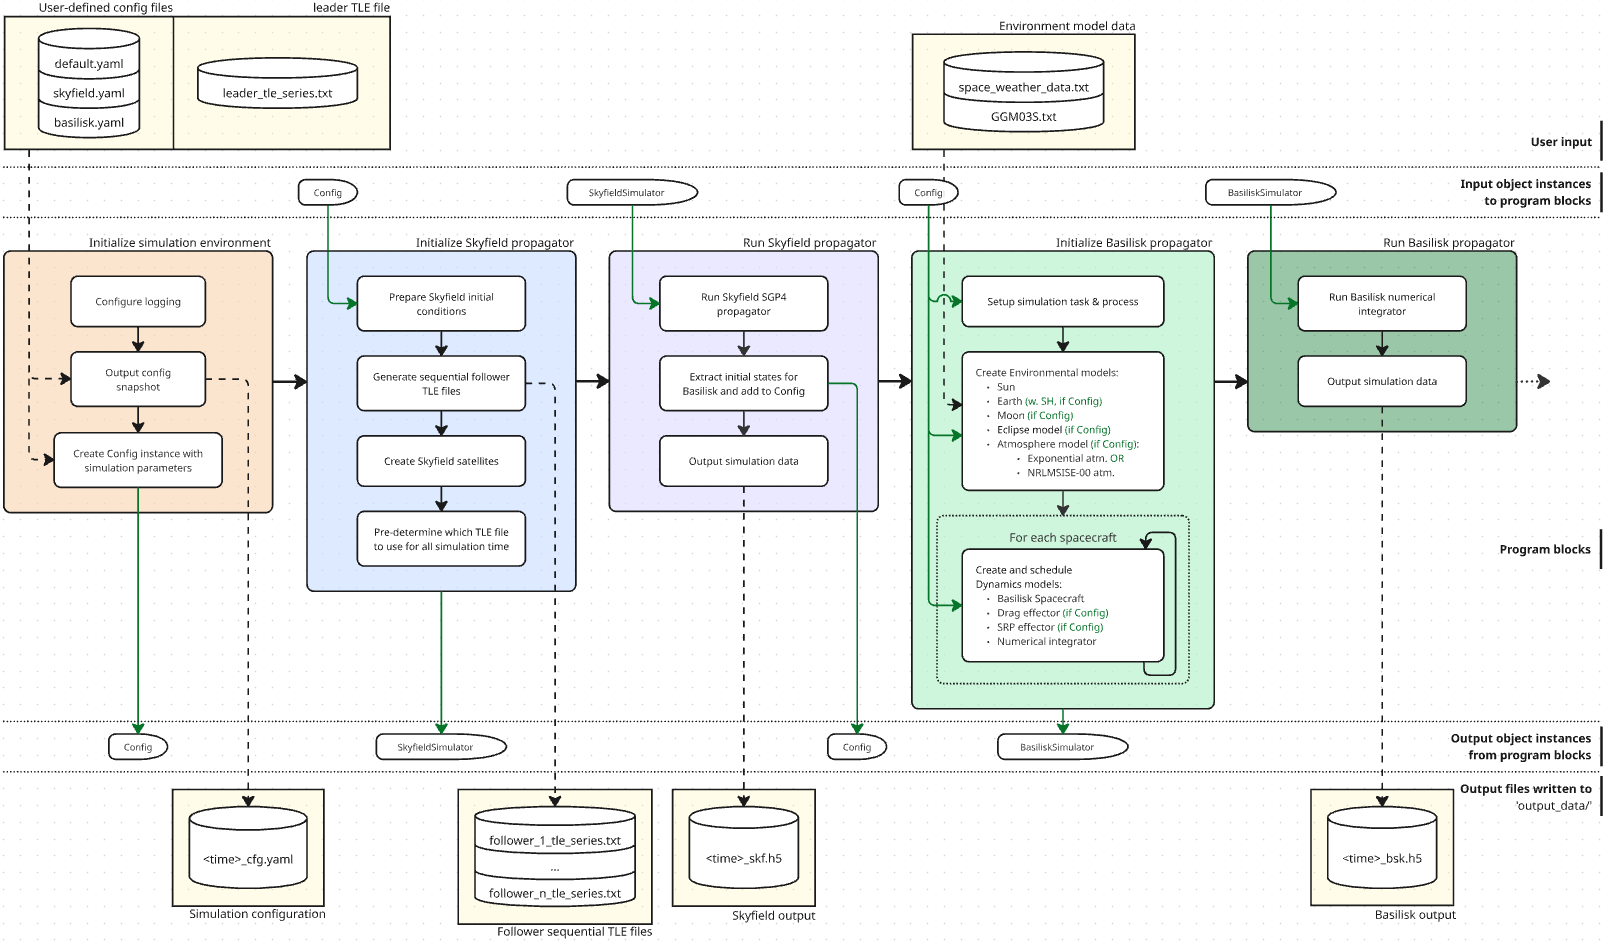
\includegraphics[width=1.3\textwidth, angle=-90]{Figures/04Method/Propagation Accuracy Comparison Simulator Flowchart v2.png}
    \caption{Full size detailed Comparative Propagation Simulator flow diagram}
    \label{fig:full_size_propagator_comp_flow} 
\end{figure}

\subsection*{GNSS-R Formation Flight Simulator}
\begin{figure}[H]
    \centering
    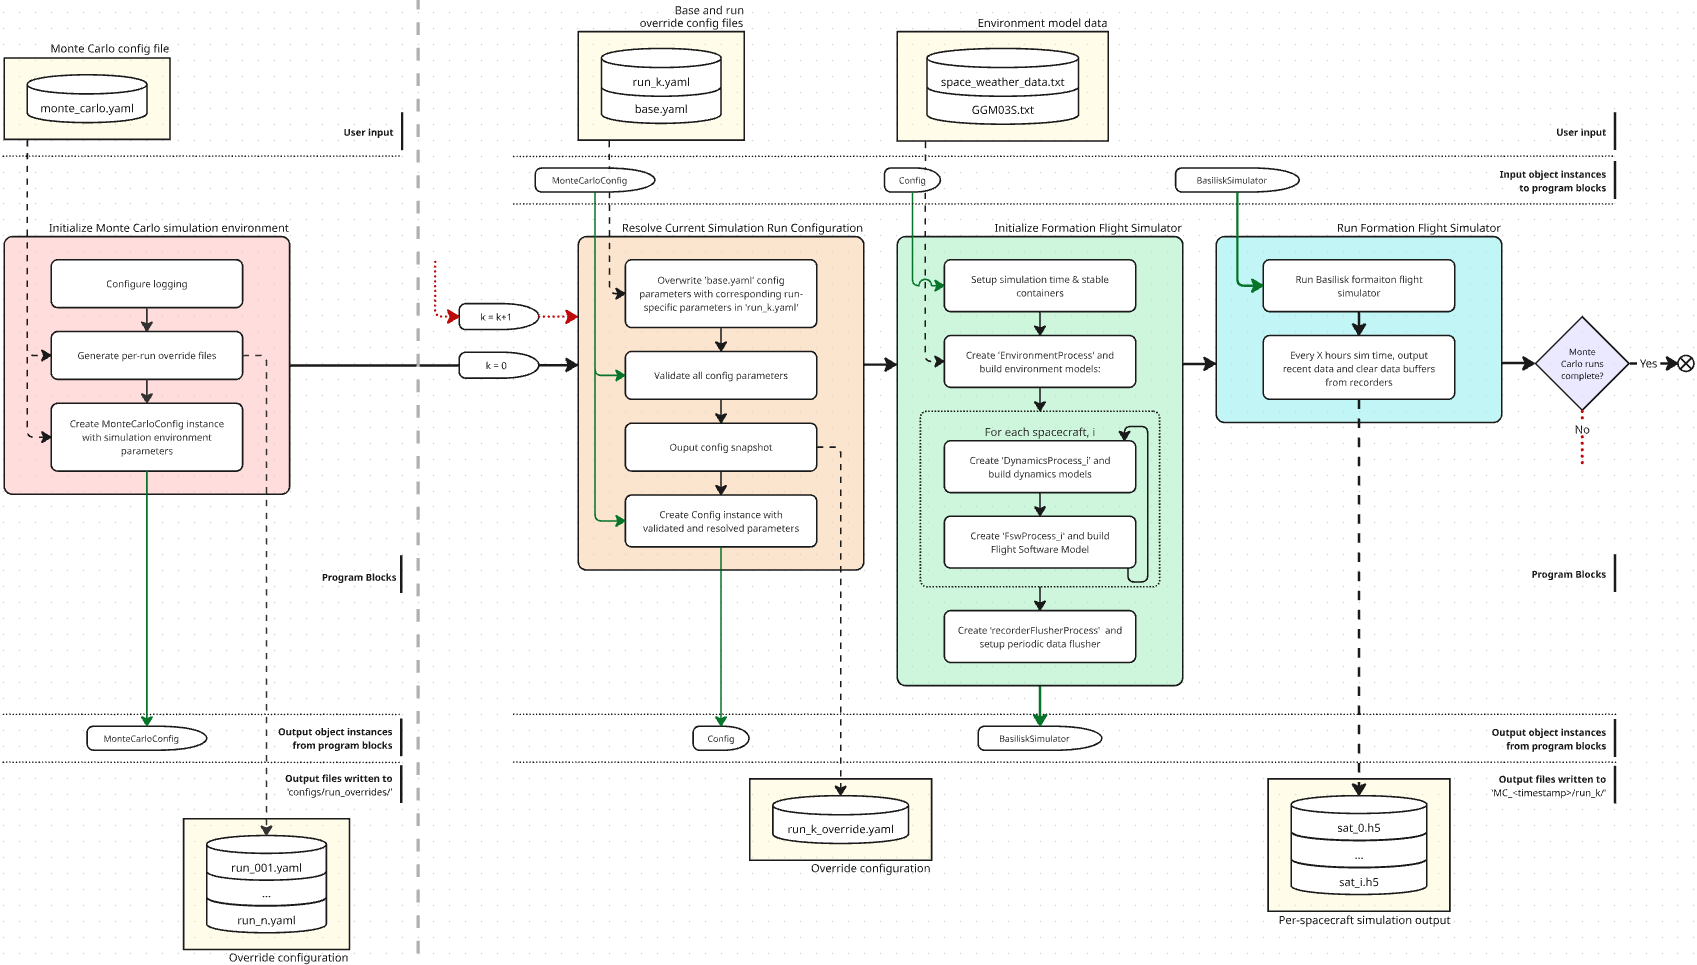
\includegraphics[width=1.4\textwidth, angle=-90]{Figures/04Method/Formation Flight Simulator.png}
    \caption{Full size detailed GNSS-R Formation Flight Simulator flow diagram}
    \label{fig:full_size_formfly_flow} 
\end{figure}


\clearpage
\section*{Simulator Basilisk Process-Task-Model Structure}

\subsection*{Comparative Propagation Simulator}
% Todo

\subsection*{GNSS-R Formation Flight Simulator}
\begin{figure}[htbp]
    \small
    \dirtree{%
    .1 GNSS-R Formation Flight Simulator.
    .2 EnvironmentProcess.
    .3 EnvironmentTask.
    .4 [20] spiceObj.
    .4 [20] eclipseObj.
    .4 [20] groundStation(s).
    .4 [20] atmObj.
    .3 MsisInputUpdaterTask.
    .4 [20] msisInputUpdater.
    .2 DynamicsProcess\_\textless sat\_idx\textgreater.
    .3 DynamicsTask\_\textless sat\_idx\textgreater.
    .4 scObj.
    .4 [20] dragEffector.
    .4 [20] srpEffector.
    .4 [20] solarPanel(s).
    .4 [20] rwEffector.
    .4 [20] thrusterEffector.
    .4 [20] fuelTankEffector.
    .4 [20] battery.
    .4 [20] obcPowerSink.
    .4 [20] rwPower(s).
    .4 [10] recorders.
    .2 FswProcess\_\textless sat\_idx\textgreater.
    .3 FswTask\_\textless sat\_idx\textgreater.
    .4 [20] scheduler.
    .4 [10] recorders.
    .2 RecorderFlusherProcess.
    .3 [20] RecorderFlusherTask.
    .4 [20] recorderFlusher.
    }
    \caption{\hl{TODO: Update and verify after simulator update. Hierarchical process-task-model structure of the GNSS-R formation flight Basilisk simulator. The number in square brackets denote the model priority, where higher priority models are updated first. Same-priority tasks are orderly updated from the top-down within a task. ``\textit{<sat\_idx>}'' represents per-spacecraft processes and tasks.}}
    \label{fig:formfly_process_hierarchy}
\end{figure}

% \clearpage
% \section*{C - Numerical Values}
% \addcontentsline{toc}{chapter}{\protect\numberline{}C - Numerical Values} 

% \section*{Numerical Values for Physical Constants}
% \begin{table}[h!]
% \centering
% \begin{tabular}{c c c}
% \hline
% $Constant$ & $Value$ & $Unit$ \\
% \hline
% $J_0$ & $-1$ & -\\
% $J_1$ & $0$ & -\\
% $J_2$ & $1.08263 \times 10^{-3}$  & -\\
% $J_3$ & $-2.53266 \times 10^{-6}$ & -\\
% $J_4$ & $-1.61962 \times 10^{-6}$ & -\\
% $P_{Sun}$ & $4.578299965 \times 10^{-6}$ & $Ws/m^3$ \\
% $1AU$ & $149597871$ & $km$ \\
% $R$ & $6378136.6$ & $m$ \\
% $H_0$ & $7200$ & $m$ \\
% $\rho_0$ & $1.225$ & $kg/m^3$ \\
% $-$ & $-$ & $-$ \\
% $-$ & $-$ & $-$ \\
% $-$ & $-$ & $-$ \\
% \hline
% \end{tabular}
% \caption{Physical constants and associated numerical value. $J$-terms courtesy of}
% \label{tab:phys_const}
% \end{table}
%%%%%%%%%%%%%%%%%%%%%%%%%%%%%%%%%%%%%%%%%%%%%%%%%%%%%%%%


% \chapter*{B - Sidenote statistics}
% \addcontentsline{toc}{chapter}{\protect\numberline{}B - Sidenote statistics} 

% %For included tables and figures renew the numbering such that they are numbered by the appendix they are attached to and not to the conclusion chapter
% \renewcommand{\thefigure}{B.\arabic{figure}}
% \setcounter{figure}{0}
% \renewcommand{\thetable}{B.\arabic{table}}
% \setcounter{table}{0}


% \section*{\large{B1 - Some random table}}
% \vspace*{1cm}

% Remember to only include one thing per page in the appendices.

% \begin{table}[ht!]
% \centering
%     \begin{tabular}{ m{4cm} m{2.5cm} m{2.5cm} m{2.5cm} } 
%     \toprule
%     \toprule
%     \textbf{Statistic} & \textbf{One} & \textbf{Two}  \\
%     \midrule
%     Count   & 387317    & 283960    \\[1.3ex]
%     Mean    & 130.66    & 134.18    \\[1.3ex]
%     Std     & 248.09    & 230.32    \\[1.3ex]
%     Q1      & 31.00     & 21.00     \\[1.3ex]
%     Median  & 67.00     & 63.00     \\[1.3ex]
%     Q3      & 142.00    & 159.00    \\[1.3ex]
%     Min     & 0.00      & 0.00      \\[1.3ex]
%     Max     & 14519.00  & 14253.00  \\[1.3ex]
%     \bottomrule
%     \bottomrule
%     \end{tabular}
% \caption[Statistics on something]{Table of statistics on some sidenote data.}
% \end{table}


% % Page without title but section title:
% \newpage
% \section*{\large{B2 - Some other random table}}
% \vspace*{1cm}

% \begin{table}[ht!]
% \centering
%     \begin{tabular}{ m{4cm} m{2.5cm} m{2.5cm} m{2.5cm} } 
%     \toprule
%     \toprule
%     \textbf{Statistic} & \textbf{Three} & \textbf{Four}  \\
%     \midrule
%     Count   & 387317    & 283960    \\[1.3ex]
%     Mean    & 130.66    & 134.18    \\[1.3ex]
%     Std     & 248.09    & 230.32    \\[1.3ex]
%     Q1      & 31.00     & 21.00     \\[1.3ex]
%     Median  & 67.00     & 63.00     \\[1.3ex]
%     Q3      & 142.00    & 159.00    \\[1.3ex]
%     Min     & 0.00      & 0.00      \\[1.3ex]
%     Max     & 14519.00  & 14253.00  \\[1.3ex]
%     \bottomrule
%     \bottomrule
%     \end{tabular}
% \caption[Statistics on something else]{Table of statistics on some other sidenote data.}
% \end{table}



% \newpage
% \section*{\large{B3 - Some random figure}}
% \vspace*{1cm}

% \begin{figure}[H]
%   \centering
%   \subfloat[Data set sizes for data X.]
%   {\includegraphics[width=1\textwidth]{Figures/dataset_X.png}}
%   \hfill
%   \subfloat[Data set sizes for data Y.]
%   {\includegraphics[width=1\textwidth]{Figures/dataset_Y.png}}
%   \caption[Data set sizes]{The figures show the data set sizes of X and Y and the proposed cut-off threshold at 10 $\%$ of the mean set size.}
% \end{figure}



%%%%%%%%%%%%%%%%%%%%%%%%%%%%%%%%%%%%%%%%%%%%%%%%%%%%%%%%
 

\end{document}